\documentclass[oneside]{book}
\usepackage{lmodern}
\usepackage[margin=1in]{geometry}
\usepackage[svgnames]{xcolor}
\usepackage[a-3u,pdf17]{pdfx}
\usepackage{hyperref}
\hypersetup{colorlinks=true,linkcolor=NavyBlue}
\usepackage[shortlabels]{enumitem}
\usepackage{mathtools}
\usepackage{booktabs}
\usepackage{nicematrix}
\usepackage{derivative}
\usepackage{etoolbox}
\usepackage{amssymb}
\usepackage{pgfplots}
\pgfplotsset{compat=1.18}
\usepgfplotslibrary{fillbetween}

% just to make sure it exists
\providecommand\given{}%
% can be useful to refer to this outside \Set
\newcommand\SetSymbol[1][]{%
    \nonscript\:#1\vert{}%
    \allowbreak%
    \nonscript\:%
    \mathopen{}}%
\DeclarePairedDelimiterXPP{\E}[1]{\operatorname{\mathbb{E}}}[]{}{%
    \renewcommand\given{\SetSymbol[\delimsize]}%
    \ifblank{#1}{\:\cdot\:}{#1}}
\DeclarePairedDelimiterXPP{\Var}[1]{\operatorname{Var}}(){}{%
    \renewcommand\given{\SetSymbol[\delimsize]}%
    \ifblank{#1}{\:\cdot\:}{#1}}
\DeclarePairedDelimiterXPP{\Cov}[1]{\operatorname{Cov}}(){}{%
    \renewcommand\given{\SetSymbol[\delimsize]}%
    \ifblank{#1}{\:\cdot\:}{#1}}
\DeclarePairedDelimiterXPP\Prob[1]{\operatorname{\mathbb{P}}}(){}{%
    \renewcommand\given{\SetSymbol[\delimsize]}%
    \ifblank{#1}{\:\cdot\:}{#1}}
\DeclarePairedDelimiterXPP\Ind[1]{\operatorname{\mathbb{I}}}\{\}{}{%
    \renewcommand\given{\SetSymbol[\delimsize]}%
    \ifblank{#1}{\:\cdot\:}{#1}}
\DeclarePairedDelimiterXPP{\GCD}[1]{\operatorname{gcd}}\{\}{}{\ifblank{#1}{\:\cdot\:}{#1}}
\DeclarePairedDelimiterXPP{\LN}[1]{\operatorname{ln}}(){}{\ifblank{#1}{\:\cdot\:}{#1}}
\DeclarePairedDelimiterXPP{\MIN}[1]{\operatorname{min}}\{\}{}{\ifblank{#1}{\:\cdot\:}{#1}}
\DeclarePairedDelimiterXPP{\MAX}[1]{\operatorname{max}}\{\}{}{\ifblank{#1}{\:\cdot\:}{#1}}
\DeclarePairedDelimiterXPP{\diag}[1]{\operatorname{diag}}(){}{\ifblank{#1}{\:\cdot\:}{#1}}
\DeclarePairedDelimiterXPP{\sign}[1]{\operatorname{sign}}(){}{\ifblank{#1}{\:\cdot\:}{#1}}
\DeclarePairedDelimiterXPP{\expit}[1]{\operatorname{expit}}(){}{\ifblank{#1}{\:\cdot\:}{#1}}
\DeclarePairedDelimiterXPP{\logit}[1]{\operatorname{logit}}(){}{\ifblank{#1}{\:\cdot\:}{#1}}
\DeclarePairedDelimiterXPP{\order}[1]{\operatorname{o}}(){}{\ifblank{#1}{\:\cdot\:}{#1}}

% Discrete Distributions
\DeclarePairedDelimiterXPP{\BERN}[1]{\text{BERN}}(){}{#1}%
\DeclarePairedDelimiterXPP{\BIN}[1]{\text{BIN}}(){}{#1}%
\DeclarePairedDelimiterXPP{\NBt}[1]{\text{NB}_t}(){}{#1}%
\DeclarePairedDelimiterXPP{\NBf}[1]{\text{NB}_f}(){}{#1}%
\DeclarePairedDelimiterXPP{\GEOt}[1]{\text{GEO}_t}(){}{#1}%
\DeclarePairedDelimiterXPP{\GEOf}[1]{\text{GEO}_f}(){}{#1}%
\DeclarePairedDelimiterXPP{\DU}[1]{\text{DU}}(){}{#1}%
\DeclarePairedDelimiterXPP{\HG}[1]{\text{HG}}(){}{#1}%
\DeclarePairedDelimiterXPP{\POI}[1]{\text{POI}}(){}{#1}%
\DeclarePairedDelimiterXPP{\MN}[1]{\text{MN}}(){}{#1}%

% Continuous Distributions
\DeclarePairedDelimiterXPP{\Uniform}[1]{\text{U}}(){}{#1}%
\DeclarePairedDelimiterXPP{\BetaDist}[1]{\text{Beta}}(){}{#1}%
\DeclarePairedDelimiterXPP{\Erlang}[1]{\text{Erlang}}(){}{#1}%
\DeclarePairedDelimiterXPP{\EXP}[1]{\text{EXP}}(){}{#1}%

\DeclarePairedDelimiterX\abs[1]\lvert\rvert{\ifblank{#1}{\:\cdot\:}{#1}}
\DeclarePairedDelimiterX\Set[1]\{\}{%
    \renewcommand\given{:}%
    #1%
}

\providecommand{\Vector}[1]{\underline{#1}}
\providecommand{\Matrix}[1]{\boldsymbol{#1}}

\usepackage{stackengine}
\usepackage[british]{isodate}
\usepackage[british]{babel}
\newcommand{\makeheading}[2]%
{%
\begin{center}%
    \makebox[\linewidth]{\raisebox{-.5ex}[0cm][0cm]{\stackanchor{\textcolor{Gray}{\textsc{#1}}}{\emph{\scriptsize\printyearoff#2}}\;}\color{Crimson!50}\hrulefill}%
\end{center}%
}%

\usepackage[breakable]{tcolorbox}
\tcbset{
    regular/.style={
        boxrule=0mm,
        breakable,
        sharp corners
    }
}

\newtcolorbox{Example}{regular,colframe=Green!20!white,colback=Green!10!white}%
\newtcolorbox{Regular}{regular,colframe=Navy!15!white,colback=Navy!5!white}%
\newtcolorbox{Result}{regular,colframe=Red!15!white,colback=Red!5!white}%

\title{%
\LARGE Stochastic Processes 1\\%
\large STAT 333\\%
\normalsize Fall 2021 (1219)\thanks{Online Course}}%
\author{Cameron Roopnarine\thanks{\LaTeX{}er}\and Steve Drekic\thanks{Main Instructor}\and Mirabelle Huynh\thanks{Assisting Instructor}}%
\date{Last updated: \today}

\usepackage{tikz}
\usetikzlibrary{petri,calc}

\begin{document}
\maketitle
\tableofcontents
\chapter{Integration}
\setcounter{section}{1}
\section{Riemann Sums and the Definite Integral}
To begin with, our goal is to develop methods for determining the area under a curve.

We know we can approximate the area using rectangles (or other geometric shapes), but
we want the \emph{exact} area. For this, we will need \emph{Riemann sums}.

\begin{Definition}{Partition}{partition}
    A \textbf{partition}, $P$, for the interval $ \interval{a}{b} $ is a finite
    sequence of increasing numbers of the form
    \[ a=t_0<t_1<t_2\cdots<t_{n-1}<t_n=b \]
    This partition subdivides the interval $ \interval{a}{b} $ into $ n $ subintervals:
    \[ \interval{t_0}{t_1},\ldots,\interval{t_{n-1}}{t_n} \]
\end{Definition}

\begin{Remark}{}{}
    These subintervals may \emph{not} all have the same length.
\end{Remark}

\begin{Definition}{Length}{length}
    Denote the \textbf{length} of the $ i^{\text{th}} $ subinterval,
    $ \interval{t_{i-1}}{t_i} $, by $ \Delta t_i $; that is, $ \Delta t_i=t_i-t_{i-1} $.
\end{Definition}

\begin{Definition}{Norm}{norm}
    The \textbf{norm} of a partition is the length of the widest subinterval:
    \[ \norm{P}=\max(\Delta t_1,\dots,\Delta t_{n}) \]
\end{Definition}

\begin{Definition}{Riemann sum}{riemann_Sum}
    Given a bounded function $ f $ on $ \interval{a}{b} $,
    a partition $ P $ of $ \interval{a}{b} $, and a set
    $ \set{c_1,\dots,c_n} $, where $ c_i\in\interval{t_{i-1}}{t_i} $, then a
    \textbf{Riemann sum} for $ f $ with respect to $ P $ is
    \[ S=\sum\limits_{i=1}^{n} f(c_i)\Delta t_i \]
\end{Definition}

Again, we want the \emph{exact} area, and for that we will need to use infinitely
many points!

But we do need to make sure that the norm of our partitions is getting smaller,
and that the area we get doesn't depend on the choice of Riemann sum.

\begin{Definition}{Integrable, Integral of $ f $}{integrable}
    We say that $ f $ is \textbf{integrable} on $ \interval{a}{b} $ if there exists a unique number
    $ I\in\mathbb{R} $ such that if whenever $ \set{P_n} $ is a sequence of partitions with
    $ \lim\limits_{{n} \to {\infty}}\norm{P_n}=0 $ and $ \set{S_n} $ is any sequence of
    Riemann sums associated to the $ P_n $'s, we have $ \lim\limits_{{n} \to {\infty}} S_n=I $.

    In this case, we call $ I $ the \textbf{integral of $ f $} over $ \interval{a}{b} $
    and denote it by
    \[ \int_{a}^{b} f(x)\, dx \]
    where $ a,b $ are the bounds of integration, $ f(x) $ is the integrand, $ x $ is the
    variable of integration. The complete object is called a definite integral.

    It represents the exact (signed) area under $ f $.
\end{Definition}

\begin{Remark}{}{}
    The variable of integration is a \emph{dummy variable} since we can change it into
    whatever we want and it won't change the value of the integral; that is,
    \[
        \int_{a}^{b} f(x)\,dx =
        \int_{a}^{b} f(t) \,d{t}=
        \int_{a}^{b} f(\cdot)\, d{\cdot}
    \]
\end{Remark}

This looks \emph{horrible} to compute in practice (and it is). The good news is if
$ f $ is continuous, it's not so bad! (still bad though)

\begin{Theorem}{Integrability Theorem for Continuous Functions}{integrability_thm}
    Let $ f $ be continuous on $ \interval{a}{b} $.
    Then $ f $ is integrable on $ \interval{a}{b} $.
\end{Theorem}

\begin{Proof}{\ref{thm:integrability_thm}}{}
    Beyond the scope of this course.
\end{Proof}

This is fantastic! This means that we can \emph{choose} any collection of Riemann sums
we want when computing the integral of a continuous function!

Let's examine a ``nice'' choice: one where the partition is regular and where we just
pick the $ c_i $'s to be the right-hand endpoints!

\begin{Definition}{Regular $n$-partition}{regular_partition}
    For the interval $ \interval{a}{b} $, the \textbf{regular $ n $-partition}
    where all $ n $ subintervals
    have the same length; that is,
    \[ \Delta t=\frac{b-a}{n} \quad\text{and}\quad  t_i=t_0+i\Delta t \]
\end{Definition}

\begin{Definition}{Regular right-hand Riemann sum}{right_hand_reimann}
    Using this, we define the \textbf{regular right-hand Riemann sum} by taking $ c_i=t_i $ for
    all $ i $:
    \[ S_n=\sum\limits_{i=1}^{n} f(t_i)\Delta t=\sum\limits_{i=1}^{n} f(t_i)\left(\frac{b-a}{n}\right) \]
\end{Definition}

\begin{Remark}{}{}
    We can also define the regular left-hand Riemann sum.
\end{Remark}

Now, we can write a nicer formula for integrating continuous functions!

If $ f $ is continuous, then
\[ \boxed{\int_{a}^{b} f(x)\, d{x} =
        \lim\limits_{{n} \to {\infty}} \sum\limits_{i=1}^{n} f(t_i)\left(\frac{b-a}{n}\right)} \]

\begin{Example}{}{}
    Evaluate
    $ \displaystyle\int_{0}^{4} x+x^3\, d{x} $.

    \textbf{Solution.}
    Since $ f(x)=x+x^3 $ is continuous, we can use the above formula.

    In our case: $ \dfrac{b-a}{n} = \dfrac{4}{n} $, and $ t_i = 0+\dfrac{4i}{n} = \dfrac{4i}{n} $.

    So, $ f(t_i) = \dfrac{4i}{n} + \dfrac{64i^3}{n^3} $.
    Then, we get:
    \begin{align}
        \int_{0}^{4} x+x^3\, d{x}
         & = \lim\limits_{{n} \to {\infty}} \sum\limits_{i=1}^{n}
        \left( \frac{4i}{n} +\frac{64i^3}{n^3} \right)\left( \frac{4}{n} \right)                  \\
         & = \lim\limits_{{n} \to {\infty}} \frac{16}{n^2} \sum\limits_{i=1}^{n} i +
        \frac{256}{n^4} \sum\limits_{i=1}^{n} i^3 \label{1.2_reimann}                             \\
         & = \lim\limits_{{n} \to {\infty}} \frac{16}{n^2} \left[ \frac{n(n+1)}{2} \right] +
        \frac{256}{n^4} \left[ \frac{n^2(n+1)^2}{4} \right] \label{1.3_reimann}                   \\
         & = \lim\limits_{{n} \to {\infty}} \frac{8n+8}{n} +64 \left(\frac{n^2+2n+1}{n^2} \right) \\
         & = 8+64                                                                                 \\
         & =72
    \end{align}
    where from~\ref{1.2_reimann} to~\ref{1.3_reimann} we used both of the following:
    \[ \sum\limits_{i=1}^{n} i=\frac{n(n+1)}{2} \text{ and }
        \sum\limits_{i=1}^{n} i^3=\frac{n^2(n+1)^2}{4} \]
\end{Example}

\begin{Remark}{}{}
    The theorem also holds for functions that are bounded and have finitely many
    discontinuities.
\end{Remark}

\section{Properties of the Definite Integral}

Since a definite integral is the limit of a sequence, many limit laws also hold!

\begin{Theorem}{Properties of Integrals}{properties_of_integrals}
    Assume that $ f $ and $ g $ are integrable on the interval $ \interval{a}{b} $. Then:
    \begin{enumerate}[label=(\arabic*)]
        \item\label{property_integral_1} For any $ c\in\mathbb{R} $,
              $ \displaystyle\int_{a}^{b} cf(x)\, d{x} = c \int_{a}^{b} f(x)\, d{x} $.
        \item\label{property_integral_2}
              $ \displaystyle \int_{a}^{b} (f+g)(x)\, d{x} = \int_{a}^{b} f(x)\, d{x} +
                  \int_{a}^{b} g(x)\, d{x} $.
        \item\label{property_integral_3} If $ m\le f(x)\le M $ for all $ x\in\interval{a}{b} $,
              then
              $ \displaystyle m(b-a)\le \int_{a}^{b} f(x)\, d{x} \le M(b-a) $.
        \item\label{property_integral_4} If $ 0\le f(x) $ for all $ x\in\interval{a}{b} $, then
              $ \displaystyle 0\le \int_{a}^{b} f(x)\, d{x} $.
        \item\label{property_integral_5} If $ f(x)\le g(x) $ for all $ x\in\interval{a}{b} $, then
              $ \displaystyle \int_{a}^{b} f(x)\, d{x} \le \int_{a}^{b} g(x)\, d{x} $.
        \item\label{property_integral_6} The function
              $ \abs{f} $ is integrable on $ \interval{a}{b} $ and
              $ \displaystyle \abs[\bigg]{\int_{a}^{b} f(x)\, d{x}}
                  \le \int_{a}^{b} \abs{f(x)}\, d{x} $.
    \end{enumerate}
\end{Theorem}

\begin{Proof}{\ref{thm:properties_of_integrals}}{}
    \begin{itemize}
        \item~\ref{property_integral_1} and~\ref{property_integral_2} follow from limit laws
              for sequences.
        \item~\ref{property_integral_3} implies~\ref{property_integral_4}.
        \item~\ref{property_integral_1},~\ref{property_integral_2},
              and~\ref{property_integral_4} imply~\ref{property_integral_5}.
        \item~\ref{property_integral_6} follows from the triangle inequality.
    \end{itemize}

    We will now prove~\ref{property_integral_3}.

    Suppose $ m\le f(x)\le M $ and partition the interval
    $ a=t_0<\cdots<t_n=b $.

    Note that
    $ \displaystyle\sum\limits_{i=1}^{n} \Delta t=\frac{b-a}{n}(n)=b-a $
    Then, since $ m\le f(x)\le M $, we get
    \[ m(b-a)=\sum\limits_{i=1}^{n} m\Delta t\le \sum\limits_{i=1}^{n} f(t_i)\Delta t
        \le \sum\limits_{i=1}^{n} M\Delta t=M(b-a) \]
    So, taking limits gives
    \[ m(b-a)\le \int_{a}^{b} f(x)\,d{x} \le M(b-a) \]
\end{Proof}

\begin{Definition}{More properties}{more_properties}
    \begin{enumerate}[label=(\Roman*)]
        \item If $ f(a) $ is defined, then
              $ \displaystyle\int_{a}^{a} f(x)\, d{x} =0 $
        \item If $ f $ is integrable on $ \interval{a}{b} $, then
              $ \displaystyle\int_{a}^{b} f(x)\, d{x}=-\int_{b}^{a} f(x)\, d{x} $
    \end{enumerate}
\end{Definition}

\begin{Theorem}{}{extra_integ_property}
    If $ f $ is integrable on an interval $ I $ containing $ a,b $, and $ c $, then
    \[ \int_{a}^{b} f(x)\, d{x}=\int_{a}^{c} f(x)\, d{x}+\int_{c}^{b} f(x)\, d{x} \]
\end{Theorem}

\begin{Proof}{\ref{thm:extra_integ_property}}{}
    Beyond the scope of this course.
\end{Proof}

\begin{Remark}{}{}
    $ c $ does \emph{not} need to be between $ a $ and $ b $!
\end{Remark}

\subsection*{Geometric Interpretation of the Integral}
So far, we have only examined positive functions, but we should note that $ \int_{a}^{b} f(x)\,dx $
returns the \emph{signed} area between $ f $ and the $ x $-axis. That is, if $ f(x)\le 0 $, then
$ \int_{a}^{b} f(x)\,dx\le 0 $ too.

So, in general, $ \int_{a}^{b} f(x)\,dx $ is the area under $ f $ that
lies above the $ x $-axis \emph{minus} the area above the graph of
$ f $ that lies below the $ x $-axis.

\begin{Example}{}{}
    \[ \int_{-1}^{1}x\,dx=R_2-R_1 \]
    but $ R_2=R_2 $, so
    \[ \int_{-1}^{1}x\,dx=0 \]
    \begin{figure}[H]
        \centering
        \tikzset{every picture/.style={line width=0.75pt}} %set default line width to 0.75pt        

        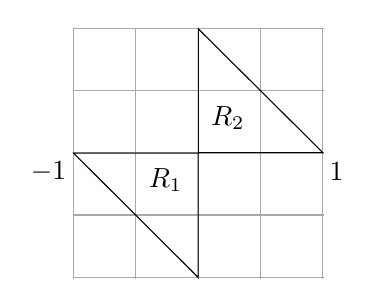
\begin{tikzpicture}[x=0.75pt,y=0.75pt,yscale=-1,xscale=1]
            %Shape: Grid [id:dp8044758903954956] 
            \draw  [draw opacity=0] (252.83,80.33) -- (373.67,80.33) -- (373.67,201.33) -- (252.83,201.33) -- cycle ; \draw  [color={rgb, 255:red, 168; green, 168; blue, 168 }  ,draw opacity=1 ] (252.83,80.33) -- (252.83,201.33)(282.83,80.33) -- (282.83,201.33)(312.83,80.33) -- (312.83,201.33)(342.83,80.33) -- (342.83,201.33)(372.83,80.33) -- (372.83,201.33) ; \draw  [color={rgb, 255:red, 168; green, 168; blue, 168 }  ,draw opacity=1 ] (252.83,80.33) -- (373.67,80.33)(252.83,110.33) -- (373.67,110.33)(252.83,140.33) -- (373.67,140.33)(252.83,170.33) -- (373.67,170.33)(252.83,200.33) -- (373.67,200.33) ; \draw  [color={rgb, 255:red, 168; green, 168; blue, 168 }  ,draw opacity=1 ]  ;
            %Shape: Right Triangle [id:dp6090851976145147] 
            \draw   (313,80.67) -- (373,140.33) -- (313,140.33) -- cycle ;
            %Shape: Right Triangle [id:dp2511359111159521] 
            \draw   (312.83,200.33) -- (252.83,140.5) -- (312.83,140.5) -- cycle ;

            % Text Node
            \draw (375,143.73) node [anchor=north west][inner sep=0.75pt]    {$1$};
            % Text Node
            \draw (231,143.4) node [anchor=north west][inner sep=0.75pt]    {$-1$};
            % Text Node
            \draw (287.83,146.73) node [anchor=north west][inner sep=0.75pt]    {$R_{1}$};
            % Text Node
            \draw (317.83,116.73) node [anchor=north west][inner sep=0.75pt]    {$R_{2}$};
        \end{tikzpicture}
    \end{figure}
\end{Example}

\begin{Remark}{}{}
    If we are lucky, we can use geometric formulas to evaluate integrals
    (see pg 26--28 in the notes). However, we are almost never this lucky\textellipsis{}
\end{Remark}

\section{Average Value of a Function}

\begin{Definition}{Average value}{avg_value}
    If $ f $ is continuous on $ \interval{a}{b} $, the \textbf{average value} of $ f $
    on $ \interval{a}{b} $ is defined as
    $ \displaystyle \frac{1}{b-a} \int_{a}^{b} f(x)\,dx $.
\end{Definition}

\subsection*{Geometric Interpretation}
\begin{Proof}{\ref{thm:avt}}{}
    If $ f $ is continuous on $ \interval{a}{b} $, EVT says there exists $ m,M\in\mathbb{R} $ such that
    $ \displaystyle m\le f(x) \le M $
    for $ x\in\interval{a}{b} $, and $ f(c_1)=m $, $ f(c_2)=M $ for some $ c_1,c_2\in\interval{a}{b} $.

    Also, we know
    \begin{align*}
        m(b-a)\le \int_{a}^{b} f(x)\, d{x} \le M(b-a)
         & \implies m\le \frac{1}{b-a} \int_{a}^{b} f(x)\, d{x} \le M       \\
         & \iff f(c_1)\le \frac{1}{b-a} \int_{a}^{b} f(x)\, d{x} \le f(c_2) \\
    \end{align*}
    IVT says there exists $ c $ between $ c_1 $ and $ c_2 $, so that
    \[ f(c)=\frac{1}{b-a} \int_{a}^{b} f(x)\, d{x} \]
\end{Proof}

\begin{Theorem}{Average Value Theorem (AVT)}{avt}
    Assume $ f $ is continuous on $ \interval{a}{b} $.
    There exists $ c\in\interval{a}{b} $ such that
    $ \displaystyle f(c)=\frac{1}{b-a} \int_{a}^{b} f(x) d{x} $.
\end{Theorem}

\begin{Remark}{}{}
    Note that this theorem holds even if $ b<a $ since
    \begin{align*}
        f(c) & =\frac{1}{a-b} \int_{b}^{a}\, f(x)dx                  \\
             & =\frac{1}{a-b}\biggl(-\int_{a}^{b} f(x)\, d{x}\biggr) \\
             & =\frac{1}{b-a} \int_{a}^{b} f(x)\, d{x}
    \end{align*}
\end{Remark}

The big problem we face now is that evaluating $ \int_{a}^{b} f(x)\, d{x} $ is
monstrously difficult for all but the simplest of functions.

IF ONLY THERE WAS A BETTER WAY\@!

(spoilers: there's a better way! It's the Fundamental Theorem of Calculus!)


\makeheading{Week 2}{\daterange{2021-09-13}{2021-09-17}}%chktex 8
\section{Module 1: Measures of Disease Frequency}
\subsection{Incidence and Prevalence Rates}
\subsubsection*{How do we measure and evaluate patterns of disease within a population?}
\begin{figure}[H]
    \centering
    \includegraphics[width=0.75\textwidth]{1.1/1.pdf}
\end{figure}
\subsubsection*{Primer on HIV/AIDS}
\begin{itemize}
    \item HIV (human immunodeficiency virus) is a virus that attack’s the body’s immune
          system.
    \item HIV is spread through sexual contact, sharing needles, and mother-to-child
          transmission during pregnancy, childbirth, or breastfeeding.
    \item Infection with HIV can lead to AIDS (acquired immunodeficiency syndrome).
    \item Individuals with AIDS are at increased risk of infection and infection-related
          cancers.
    \item Currently, no cure exists, but antiretroviral therapy can slow the progression of the
          disease.
\end{itemize}
\subsubsection*{1.1 Incidence and Prevalence Rates}
\begin{Regular}
    \textcolor{Blue}{Goal}: How do we measure and evaluate patterns of disease within a population?
\end{Regular}
\begin{itemize}
    \item \textcolor{Blue}{Prevalence}: The proportion of the population currently affected by a disease.
    \item \textcolor{Blue}{Incidence}: The rate at which new cases of a disease develop in a population.
\end{itemize}
\subsubsection*{Number of people living with HIV/AIDS 1990--2017}
\begin{figure}[H]
    \centering
    \includegraphics[width=0.75\textwidth]{1.1/2.pdf}
\end{figure}
\subsubsection*{Prevalence}
\textcolor{Blue}{Prevalence}: The proportion of the population currently affected by a disease.
\begin{Regular}
    \[ \begin{tabular}{>{\bfseries}c}
            Point Prevalence \\
            per 1000
        \end{tabular}=\frac{\begin{tabular}{>{\bfseries}c}
                Number of cases (new and pre-existing) in the \\
                population at a fixed point in time
            \end{tabular}}{\begin{tabular}{>{\bfseries}c}
                Number of individuals in the \\
                population at a fixed point in time
            \end{tabular}}\times 1000.  \]
\end{Regular}
\begin{Regular}
    \[ \begin{tabular}{>{\bfseries}c}
            Period Prevalence \\
            per 1000
        \end{tabular}=\frac{\begin{tabular}{>{\bfseries}c}
                Number of cases (new and pre-existing) in the \\
                population over a given time period
            \end{tabular}}{\begin{tabular}{>{\bfseries}c}
                Number of individuals in the \\
                population over a given time period
            \end{tabular}}\times 1000.  \]
\end{Regular}
\subsubsection*{Prevalence of HIV/AIDS 1990--2017}
\begin{figure}[H]
    \centering
    \includegraphics[width=0.75\textwidth]{1.1/3.pdf}
\end{figure}
\subsubsection*{Annual new cases of HIV infection, 1990--2017}
\begin{figure}[H]
    \centering
    \includegraphics[width=0.75\textwidth]{1.1/4.pdf}
\end{figure}
\subsubsection*{Cumulative Incidence}
\textcolor{Blue}{Incidence}: The rate at which \textbf{new cases} of a disease develop in a \textbf{population} over a
specific \textbf{time} period.
\begin{Regular}
    \[ \begin{tabular}{>{\bfseries}c}
            Cumulative Incidence \\
            per 1000
        \end{tabular}=\frac{\begin{tabular}{>{\bfseries}c}
                Number of new cases in the \\
                population over the time period of interest
            \end{tabular}}{\begin{tabular}{>{\bfseries}c}
                Number of individuals at risk in the \\
                population at the start of the time period of interest
            \end{tabular}}\times 1000.  \]
\end{Regular}
\begin{itemize}
    \item Assumes all subjects remain in the population and at risk for the entire time period.
    \item Easily violated: Births, deaths, immigration, emigration, case diagnosis.
    \item Consider two ways to refine the denominator calculation.
          \begin{enumerate}[1.]
              \item Use a mid-interval population estimate.
              \item Calculate the total person-time at risk in the population.
          \end{enumerate}
\end{itemize}
\subsubsection*{Incidence Density or Incidence Rate}
\begin{Regular}
    \[ \begin{tabular}{>{\bfseries}c}
            Incidence Density \\
            per 1000
        \end{tabular}=\frac{\begin{tabular}{>{\bfseries}c}
                Number of new cases in the \\
                population over the time period of interest
            \end{tabular}}{\begin{tabular}{>{\bfseries}c}
                Mid-interval estimate of the population
            \end{tabular}}\times 1000.  \]
\end{Regular}
\begin{Example}
    \begin{itemize}
        \item 3,218 new cases of HIV in Canada, 2016.
        \item 36,264,604 July 1, 2016 Canadian population estimate.
              \[ \begin{tabular}{>{\bfseries}c}
                      Incidence Density \\
                      per 100,000
                  \end{tabular}=\frac{3,218}{36,264,604}\times 100,000=8.873666. \]
        \item \emph{The incidence of HIV infection in Canada in the year 2016 was 8.87 cases per
                  100,000 persons}.
    \end{itemize}
\end{Example}
\subsubsection*{Incidence of HIV per 1,000 uninfected adults, 2000--2017}
\begin{figure}[H]
    \centering
    \includegraphics[width=0.75\textwidth]{1.1/5.pdf}
\end{figure}
\subsubsection*{Person-time at risk}
\begin{itemize}
    \item To account for varying time periods of risk we consider an alternative denominator
          for our incidence calculation.
    \item Person-time at risk is the duration of time an individual is at risk for developing
          a disease.
    \item Assuming they are initially disease free, it is the length of time from baseline until
          the first of:
          \begin{enumerate}[1.]
              \item They develop the disease of interest and become a case.
              \item They cease to be at risk of becoming a case due to either death from unrelated
                    causes or they leave the population.
              \item The end of the time period of interest is reached.
          \end{enumerate}
    \item Total person-time at risk is the sum of the individual contributions over the
          population.
\end{itemize}
\subsubsection*{Incidence Density or Incidence Rate}
\begin{Regular}
    \[ \begin{tabular}{>{\bfseries}c}
            Incidence Density \\
            per 1000
        \end{tabular}=\frac{\begin{tabular}{>{\bfseries}c}
                Number of new cases in the \\
                population over the time period of interest
            \end{tabular}}{\begin{tabular}{>{\bfseries}c}
                Mid-Total person-time at risk in the \\
                population over the time period of interest
            \end{tabular}}\times 1000.  \]
\end{Regular}
\begin{itemize}
    \item Incidence density estimate is more precise than cumulative incidence, but may be
          harder to get information needed, so this measure is often used for small
          populations.
    \item Expressed as per $10^x$ person-years (-month, -day).
\end{itemize}
\subsubsection*{Relationship Between Incidence and Prevalence}
\begin{figure}[H]
    \centering
    \includegraphics[width=0.25\textwidth]{1.1/6.jpg}
\end{figure}
\subsubsection*{Relationship Between Incidence and Prevalence}
\begin{itemize}
    \item \textbf{Incidence}: the rate new cases are diagnosed in a population.
    \item \textbf{Prevalence}: the proportion of the population currently affected by the disease.
\end{itemize}
\begin{Regular}
    \[ \textbf{Prevalence}\approx \textbf{Incidence}\times \textbf{Disease Duration} \]
\end{Regular}
\begin{itemize}
    \item Relationship is approximate but generally holds well if prevalence is low ($<10\,$\%)
          and duration is fairly constant (or an average can be taken).
    \item Note: units must be consistent in order to perform the multiplication operation.
\end{itemize}
\subsubsection*{Prevalence, new cases, and mortality for HIV/AIDS}
\begin{figure}[H]
    \centering
    \includegraphics[width=0.75\textwidth]{1.1/7.pdf}
\end{figure}
\subsubsection*{Exercise: Incidence and Prevalence Calculations}
Total population size of 100. Histories of 12 subjects with disease are below. Subjects
13--100 do not have the disease during the year of study. ($ \triangle $ Diagnosis; $ \times $ Death)
\begin{table}[H]
    \centering
    \begin{tabular}{ccc}
        \toprule
        \textbf{Subject} & \textbf{Diagnosis} $ \triangle $ & \textbf{Death} $ \times $ \\
        \midrule
        1                & $<$ January 1                                                \\
        2                & $<$ January 1                    & April 30                  \\
        3                & $<$ January 1                                                \\
        4                & $<$ January 1                                                \\
        5                & $<$ January 1                    & June 30                   \\
        6                & March 1                          & October 31                \\
        7                & May 1                                                        \\
        8                & May 1                                                        \\
        9                & July 1                                                       \\
        10               & July 1                           & October 31                \\
        11               & NA                               & May 1                     \\
        12               & NA                               & September 1               \\
        13--100          & NA                                                           \\
        \bottomrule
    \end{tabular}
\end{table}
\begin{figure}[H]
    \centering
    \includegraphics[width=0.75\textwidth]{1.1/8.pdf}
\end{figure}
\begin{itemize}
    \item Point Prevalence on July 1.
    \item Period Prevalence (Jan 1 to Dec 31)
    \item Cumulative Incidence (Jan 1 to Dec 31).
    \item Incidence Density (Jan 1 to Dec 31).
\end{itemize}
\begin{align*}
    \begin{tabular}{c}
        Point Prevalence \\
        on July 1
    \end{tabular}
     & =\frac{\text{\# cases in the pop on July 1}}{\text{\# indv in the pop on July 1}}\times 1000=\frac{8}{97}\times 1000=\text{$82.47$ per 1000 persons}.                     \\\\
    \begin{tabular}{c}
        Period Prevalence \\
        (Jan 1-Dec 31)
    \end{tabular}
     & =\frac{\text{\# cases during Jan 1-Dec 31}}{\text{\# indv in the pop Jan 1-Dec 31}}\times 1000=\frac{10}{100}\times 1000=\text{$100$ per 1000 persons}.                   \\\\
    \begin{tabular}{c}
        Cumulative Incidence \\
        (Jan 1-Dec 31)
    \end{tabular}
     & =\frac{\text{\# new cases during Jan 1-Dec 31}}{\text{\# indv at risk on Jan 1}}\times 1000=\frac{5}{95}\times 1000=\text{$52.63$ per 1000 persons}.                      \\\\
    \begin{tabular}{c}
        Incidence Density \\
        (Jan 1-Dec 31)
    \end{tabular}
     & =\frac{\text{\# new cases during Jan 1-Dec 31}}{\text{July 1 population size}}\times 1000=\frac{5}{97}\times 1000=\text{$51.55$ per 1000 persons}.                        \\\\
    \begin{tabular}{c}
        Incidence Density \\
        (Jan 1-Dec 31)
    \end{tabular}
     & =\frac{\text{\# new cases during Jan 1-Dec 31}}{\text{\small Total person-years at risk Jan 1-Dec 31}}\times 1000=\frac{5}{90.83}\times 1000=\text{$55.05$ per 1000 p-y}. \\
\end{align*}
\subsection{Standardization of Rates: Indirect Methods}
% Chapter 2 Part 1
\chapter{Causal Inference and Potential Outcomes}
\makeheading{Week 3}{\daterange{2022-01-17}{2022-01-21}}%chktex 8
\section{Causal Inference}
\subsection{Introduction}
\subsubsection{Reference}
\begin{itemize}
    \item Hernán M.A., \& Robins J.M. (2020). Causal Inference: What
          If. Boca Raton: Chapman Hall/CRC\@.

          \url{https://www.hsph.harvard.edu/miguel-hernan/
              causal-inference-book/}
\end{itemize}
\subsubsection{Causal Inference}
Two notions of causation:
\begin{itemize}
    \item Causes of an effect/outcome.
    \item Effects of a cause.
\end{itemize}
\textbf{Causes of an effect}
\begin{itemize}
    \item What are causes of lung cancer?
    \item What was the cause of outbreak of food poisoning?
\end{itemize}
\textbf{Effects of a cause/intervention}
\begin{itemize}
    \item Does smoking cause lung cancer?
    \item Does mixed feeding cause obesity?
    \item How strong is the effect?
\end{itemize}
\begin{itemize}
    \item We concentrate on effects of a cause/treatment/intervention.
    \item Fundamentally simpler question: search is for useful
          information rather than complete scientific understanding.
    \item Typical approach for estimating causal effects (which may be
          problematic):
          collect sample on treatments/exposures, outcomes, and other
          variables in population; Use standard statistical methods
          (such as multiple regression) to derive inferences about
          associations between observable variables.
\end{itemize}
\subsubsection*{A Note}
\begin{itemize}
    \item In pharmaceutical companies, people used to believe
          conducting randomized clinical trials is the only way to
          evaluate a newly developed drug. However, there is a shifting
          trend going on right now because of:
          \begin{itemize}
              \item Difficult to find control subjects.
              \item Compliance issue.
              \item Exclusion criteria.
              \item Cost issue.
          \end{itemize}
    \item New trend: utilizing existing Electronic Health Records data
          to help find controls.
    \item The study is not randomized any more: observational study.
\end{itemize}
\subsubsection*{Draw Causality}
\textbf{Observational Studies}
\begin{itemize}
    \item No control over which subjects have the exposure and which
          do not.
    \item Exposed and Unexposed groups may be quite different with
          respect to other subject characteristics
    \item It is sometimes useful to use these studies to look at the
          natural history of a disease, but any attempt to identify
          causality b/t a risk factor and outcome must be done w/
          great caution.
\end{itemize}
\subsection{Confounding}
\subsubsection*{Confounding Issue in Observational Studies}
\begin{Example}{}
    Differences in the outcome are not only due to the treatment, but
    also because of the masking effect of covariates (confounders).
    \begin{center}
        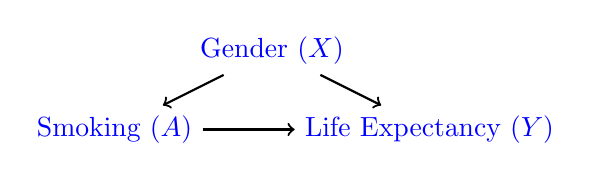
\begin{tikzpicture}[thick]
            \node (1) at (0,1) {\textcolor{Blue}{Gender ($ X $)}};
            \node (2) at (-2,0) {\textcolor{Blue}{Smoking ($ A $)}};
            \node (3) at (2,0) {\textcolor{Blue}{Life Expectancy ($ Y $)}};
            \draw[->] (1) to (2);
            \draw[->] (1) to (3);
            \draw[->] (2) to (3);
        \end{tikzpicture}
    \end{center}
    Here, gender is known as a confounder. Very often, in real
    applications, the list of potential confounders could be very large,
    and even high-dimensional.
\end{Example}
\subsubsection*{Another Example of Confounding}
\begin{Example}{}
    Researchers find when the consumption of ice cream increases, the
    death from drowning increases. Does eating ice cream lead to
    drowning?
    \begin{center}
        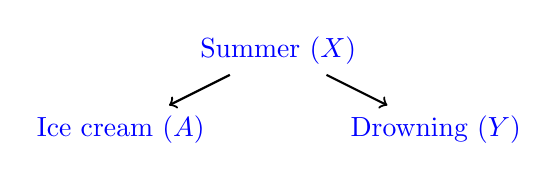
\begin{tikzpicture}[thick]
            \node (1) at (0,1) {\textcolor{Blue}{Summer ($ X $)}};
            \node (2) at (-2,0) {\textcolor{Blue}{Ice cream ($ A $)}};
            \node (3) at (2,0) {\textcolor{Blue}{Drowning ($ Y $)}};
            \draw[->] (1) to (2);
            \draw[->] (1) to (3);
        \end{tikzpicture}
    \end{center}
    Here, summer (hot weather) is a confounder.
\end{Example}
\subsubsection*{Potential Outcomes Framework}
\begin{itemize}
    \item Useful to have more precise definitions of causal effects.
    \item Demystifies the process of going from association to causation.
    \item Allows explicit statements regarding what assumptions are
          necessary to justify causal inferences.
    \item Allows for more critical, better informed evaluation of causal
          claims.
    \item Helps determine when familiar methods useful or unfamiliar
          methods necessary.
    \item Motivates derivation and use of unfamiliar methods.
\end{itemize}
\section{Potential Outcomes Framework}
\subsection*{Definition of a Causal Effect}
\begin{Regular}{}
    Suppose we have data on subjects $ i=1,\ldots,n $.
    \begin{itemize}
        \item $ \Vector{X}_i=(\Vector{X}_{i1},\Vector{X}_{i2},\ldots,\Vector{X}_{ip})^\top $: baseline covariates/potential confounders.
        \item $ A_i $: treatment assignment/exposure status for subject $ i $
              \[ A_i=\begin{cases*}
                      1, & if exposed/treated,   \\
                      0, & if unexposed/treated.
                  \end{cases*} \]
        \item $ Y_i $: observed outcome for subject $ i $.
    \end{itemize}
    \textbf{Counterfactuals/Potential outcomes}
    \begin{itemize}
        \item $ Y_i^1 $: the potential outcome if subject $ i $ were \textcolor{Blue}{treated/exposed}.
        \item $ Y_i^0 $: the potential outcome if subject $ i $ were \textcolor{Blue}{untreated/unexposed}.
    \end{itemize}
\end{Regular}
\begin{Regular}{}
    The \textbf{individual-level causal effect} for subject $ i $ is:
    \[ Y_i^1-Y_i^0. \]
\end{Regular}
\begin{Regular}{Causal Estimand}
    The \textbf{average causal effect} (ACE) is:
    \[ \ACE=\E{Y_i^1-Y_i^0}=\E{Y_i^1}-\E{Y_i^0}, \]
    where
    \begin{itemize}
        \item $ \E{Y_i^1} $ is the mean potential outcome had all subjects in the population
              were treated/exposed, and
        \item $ \E{Y_i^0} $ is the mean potential outcome had all subjects in the population were untreated/unexposed.
    \end{itemize}
    \tcblower{}
    If $ Y $ is binary,
    \begin{itemize}
        \item ACE is causal excess risk (omit subscript $ i $):
              \[ \E{Y^1-Y^0}=\E{Y^1}-\E{Y^0}=\Prob{Y^1=1}-\Prob{Y^0=1}. \]
        \item \textbf{Causal relative risk}:
              \[ \frac{\Prob{Y^1=1}}{\Prob{Y^0=1}}. \]
        \item \textbf{Causal odds ratio}:
              \[ \frac{\Prob{Y^1=1}/\Prob{Y^1=0}}{\Prob{Y^0=1}/\Prob{Y^0=0}}. \]
        \item \textbf{Crude excess risk}:
              \[ \Prob{Y=1\given A=1}-\Prob{Y=1\given A=0}. \]
        \item \textbf{Crude relative risk}:
              \[ \frac{\Prob{Y=1\given A=1}}{\Prob{Y=1\given A=0}}. \]
        \item \textbf{Crude odds ratio}:
              \[ \frac{\Prob{Y=1\given A=1}/\Prob{Y=0\given A=1}}{\Prob{Y=1\given A=0}/\Prob{Y=0\given A=0}}. \]
    \end{itemize}
\end{Regular}
\subsection*{A Toy Example}
\begin{Example}{}
    Assume we have a population of 8 subjects:
    \[ \begin{array}{cccc}
                  & A & Y^0 & Y^1 \\
            \midrule
            S_{1} & 0 & 0   & 1   \\
            S_{2} & 0 & 1   & 1   \\
            S_{3} & 0 & 0   & 0   \\
            S_{4} & 0 & 0   & 0   \\
            S_{5} & 1 & 0   & 0   \\
            S_{6} & 1 & 1   & 0   \\
            S_{7} & 1 & 1   & 1   \\
            S_{8} & 1 & 0   & 1   \\
            \bottomrule
        \end{array} \]
    We get
    \[ \text{Causal excess risk (ACE)} =\Prob{Y^1=1}-\Prob{Y^0=1}=\frac{4}{8}-\frac{3}{8}=\frac{1}{8}. \]
    For crude excess risk, we have
    \[ \begin{array}{ccccc}
                  & A & Y^0 & Y^1 & Y \\
            \midrule
            S_{1} & 0 & 0   & 1   & 0 \\
            S_{2} & 0 & 1   & 1   & 1 \\
            S_{3} & 0 & 0   & 0   & 0 \\
            S_{4} & 0 & 0   & 0   & 0 \\
            S_{5} & 1 & 0   & 0   & 0 \\
            S_{6} & 1 & 1   & 0   & 0 \\
            S_{7} & 1 & 1   & 1   & 1 \\
            S_{8} & 1 & 0   & 1   & 1 \\
            \bottomrule
        \end{array} \]
    \[ \text{Crude excess risk}=\Prob{Y=1\given A=1}-\Prob{Y=1\given A=0}=\frac{2}{4}-\frac{1}{4}=\frac{1}{4}. \]
\end{Example}
\subsection*{Fundamental Problem of Causal Inference}
\begin{Regular}{}
    For subject $ i $, we only get to observe one of $ Y_i^1 $ and $ Y_i^0 $, that is,
    \[ Y_i=Y_i^1A_i+Y_i^0(1-A_i). \]
    \tcblower{}
    \underline{Remarks}:
    \begin{enumerate}[(1)]
        \item In the literature, the above equality is often referred as the
              consistency assumption for causal inference
        \item For each subject $i$, one of the two potential outcomes is
              always missing.
        \item For this reason, many people believe causal inference is
              essentially a missing data problem.
    \end{enumerate}
\end{Regular}
\section{Estimation}
\begin{Regular}{}
    In \textbf{randomized studies}:
    \begin{itemize}
        \item $ \E{Y\given A=1}=\E{Y^1\given A=1}=\E{Y^1} $, and
        \item $ \E{Y\given A=0}=\E{Y^0\given A=0}=\E{Y^0} $.
    \end{itemize}
    Consequently, an unbiased estimate of ACE is:
    \begin{align*}
        \widehat{\ACE}
         & =\estE{Y^1}-\estE{Y^0}                                                                                   \\
         & =\estE{Y\given A=1}-\estE{Y\given A=0}                                                                   \\
         & =\frac{\sum_{i=1}^{n}Y_i A_i}{\sum_{i=1}^{n}A_i}-\frac{\sum_{i=1}^{n}Y_i(1-A_i)}{\sum_{i=1}^{n}(1-A_i)},
    \end{align*}
    where
    \begin{itemize}
        \item $ \sum_{i=1}^{n}A_i=n_1 $ is the number of treated/exposed subjects in the sample, and
        \item $ \sum_{i=1}^{n}(1-A_i)=n_0 $ is the number of untreated/unexposed subjects in the sample.
    \end{itemize}
\end{Regular}
\begin{Regular}{}
    In \textbf{observational studies}:
    \begin{itemize}
        \item $ \E{Y\given A=1}=\E{Y^1\given A=1}\ne\E{Y^1} $, and
        \item $ \E{Y\given A=0}=\E{Y^0\given A=0}\ne\E{Y^0} $,
    \end{itemize}
    where the inequalities are due to selection bias.
    Therefore, the estimator in randomized studies is biased for ACE in
    observational studies.
\end{Regular}
\section*{Assumptions for Causal Inference}
\section{Assumption 1}
\begin{Regular}{Assumption 1: Strongly Ignorable Treatment Assignment (SITA)}
    \[ (Y^0,Y^1)\indep (A\mid X). \]
    \tcblower{}
    \underline{Remarks}:
    \begin{itemize}
        \item In observational studies, it means $X$ includes all possible
              confounders (no unmeasured confounders).
        \item In randomized studies, we have $ (Y^0,Y^1)\indep A $.
        \item Within a subset of subjects with similar $X$, exposure/treatment
              can be viewed as if it were randomly assigned.
        \item This assumption cannot be verified on the observed data;
              more plausible as the size of $X$ grows.
        \item If violated, instrumental variable approach can be used in
              some cases.
    \end{itemize}
\end{Regular}
\section{Assumptions 2--4}
\begin{Regular}{Assumption 2: Stable Unit Treatment Value Assumption (SUTVA)}
    \[ (Y_i^0,Y_i^1)\indep A_j\text{ for $i\ne j$}. \]
    \tcblower{}
    \underline{Remarks}:
    \begin{itemize}
        \item Each subject's potential outcomes are not influenced by the
              actual treatment status of other subjects.
        \item Counter-example: infectious disease, family studies.
        \item If violated, divide the subjects into clusters.
    \end{itemize}
\end{Regular}
\begin{Regular}{Assumption 3: Common Support Condition (CSC)}
    \[ 0<\Prob{A=1\given X=x}<1\text{ for any $x$}. \]
    \tcblower{}
    \underline{Remarks}:
    \begin{itemize}
        \item It means that $ Y^0 $ and $ Y^1 $ should both exist in principle.
        \item Can be violated if a particular group of subjects in the
              population always receive the treatment or never receive the
              treatment.
        \item If violated, re-define the population (exclude those subjects).
    \end{itemize}
\end{Regular}
\begin{Regular}{Assumption 4: Consistency}
    \[ Y=Y^1 A+Y^0(1-A). \]
    \tcblower{}
    \underline{Remarks}:
    \begin{itemize}
        \item The observed outcome for a subject equals to the potential
              outcome under the actual treatment assignment the subject
              receives.
        \item Can be violated if different versions of treatment have
              different causal effects.
    \end{itemize}
\end{Regular}
\section{Propensity Scores}
\subsection*{Motivation for Propensity Scores}
The SITA assumption $(Y^0,Y^1)\indep (A\mid X)$ gives us some ideas about how to
estimate causal effects for observational studies.
\begin{itemize}
    \item If we condition on $X$, we can estimate the causal effect as in a
          randomized study, which is relatively straightforward.
    \item  However, if $X$ contains a large number of covariates,
          conditioning on $X$ is challenging (curse of dimensionality).
    \item  Solution: propensity score methods
\end{itemize}
\begin{Regular}{}
    \textbf{Propensity score} is the conditional probability of being exposed/treated given baseline covariates:
    \[ \ps{x}=\Prob{A=1\given X=x}. \]
    Also,
    \[ \ps{X}=\Prob{A=1\given X}. \]
    \tcblower{}
    \underline{Remarks}:
    \begin{itemize}
        \item In simple randomized studies, $ \ps{x}=0.5 $.
        \item In observational studies, $ \ps{x} $ is unknown and must be estimated.
    \end{itemize}
\end{Regular}
\subsection*{Properties}
\subsubsection*{Properties of Propensity Score}
\begin{itemize}
    \item Propensity score is a balancing score:
          \[ X\indep (A\mid \ps{X}) \]
    \item If the treatment is strongly ignorable given $ X $, that is,
          \[ (Y^0,Y^1)\indep (A\mid X), \]
          then it is strongly ignorable given $ \ps{x} $
          \[ (Y^0,Y^1)\indep (A\mid \ps{X}). \]
    \item $ \ps{x} $ is a scalar, free of dimension of $ X $.
    \item It is a summary of the contribution of all baseline characteristics to the exposure/treatment assignment.
\end{itemize}
\section{Properties of Propensity Score}
\begin{Result}{}
    The propensity score is a \textbf{balancing score}, that is,
    \[ X\indep(A\mid \ps{X}) \]
    \tcblower{}
    \textbf{Proof}: Rosenbaum and Rubin (1983).
    \begin{align*}
        \Prob[\big]{A=1\given \ps{X},X}
         & =\Prob{A=1\given X} &  & \text{$\ps{X}$ is a function of $X$} \\
         & =\ps{X}.
    \end{align*}
    On the other hand,
    \begin{align*}
        \Prob[\big]{A=1\given \ps{X}}
         & =\E[\big]{A\given \ps{X}}                                                  &  & \text{since $A$ is binary}    \\
         & =\E[\big]{\E{A\given \underbrace{X}_{C_1}}\given\underbrace{\ps{X}}_{C_2}} &  & \text{LIE since $C_2=f(C_1)$} \\
         & =\E[\big]{\ps{X}\given \ps{X}}                                                                                \\
         & =\ps{X}.
    \end{align*}
    Therefore,
    \[ \Prob[\big]{A=1\given \ps{X},X}=\Prob[\big]{A=1\given \ps{X}}. \]
    In other words, $ X\indep (A\mid \ps{X}) $.
\end{Result}
\begin{Result}{}
    If $ (Y^0,Y^1)\indep (A\mid X) $, then
    \[ (Y^0,Y^1)\indep(A\mid \ps{X}). \]
    \tcblower{}
    \textbf{Proof}:
    \begin{align*}
        \Prob{A=1\given Y^0,Y^1,\ps{X}}
         & =\E{A\given Y^0,Y^1,\ps{X}}                                                                 &  & \text{since $A$ is binary}      \\
         & =\E[\big]{\E{A\given \underbrace{Y^0,Y^1,X}_{C_1}}\given \underbrace{Y^0,Y^1,\ps{X}}_{C_2}} &  & \text{LIE since $C_2=f(C_1)$}   \\
         & =\E[\big]{\E{A\given X}\given Y^0,Y^1,\ps{X}}                                               &  & \text{SITA}                     \\
         & =\E[\big]{\ps{X}\given Y^0,Y^1,\ps{X}}                                                                                           \\
         & =\ps{X}                                                                                                                          \\
         & =\Prob[\big]{A=1\given \ps{X}}.                                                             &  & \text{from the previous result}
    \end{align*}
    Therefore,
    \[ (Y^0,Y^1)\indep(A\mid \ps{X}). \]
\end{Result}
\chapter{ARIMA Models Continued}
\section{Stationary Process Forecasting}
Suppose we observe a time series
$ X_1,\ldots,X_T $
that we believe has been generated by an underlying
stationary process. We would like to
produce an $ h $-step ahead
forecast
\[ \hat{X}_{T+h}=\hat{X}_{T+h\mid T}=f(X_t,\ldots,X_1) \]
forecasting $ X_{T+h} $. Ideally, $ \hat{X}_{T+h} $
would minimize the prediction error
\[ L(X_{T+h},\hat{X}_{T+h})=\min_f
    L(X_{T+h},f(X_{T},\ldots,X_1)) \]
where $ L $ is a loss function.

Frequently, the loss function is taken
to be the \emph{mean-squared error} (MSE)
\[ L(X_{T+h},\hat{X}_{T+h})=
    \E[\big]{(X_{T+h}-\hat{X}_{T+h})^2} \]
When using MSE, it is natural to consider
\[ L^2=\set{\text{Random variables } X: \E{X^2}<\infty} \]
$ L^2 $ is a Hilbert space when equipped
with the inner product
\[ \innerp{X}{Y}=\E{XY} \]
Hilbert spaces are generalizations of Euclidean space ($ \mathbf{R}^d $)
in which the geometry and notation of projection
are preserved.
\[ \text{Proj}(X\to Y)=\innerp{X}{Y}Y \]
\begin{Theorem}{Projection Theoren}{}
    We say $ M\subseteq L^2 $
    is a \textbf{closed linear subspace}, if
    \begin{itemize}
        \item Linearity: $ X,Y\in M $, $ \alpha,\beta\in\mathbf{R} $
              then $ \alpha X+\beta Y\in M $
        \item Closed: If $ X_n\to X $ ($ \E{(X_n-X)^2} $),
              and $ X_n\in M $, then $ X\in M $.
    \end{itemize}
    If $ M $ is a closed linear subspace in $ L^2 $
    and $ x\in L^2 $, then there exists a
    unique $ \hat{X}\in M $ such that
    \[ \E{(X-\hat{X})^2}=\inf_{y\in M}\E{(X-Y)^2} \]
    Moreover, $ \hat{X} $ satisfies the prediction equations/normal
    equations:
    \[ (X-\hat{X})\in M^\perp \implies \E{(X-\hat{X})Y}=0\quad (\forall y\in M) \]
\end{Theorem}
In MSE forecasting, we want to choose
$ \hat{X}_{T+h} $ satisfying
\[ \E{(X_{T+h}-\hat{X}_{T+h})^2}=\inf_{y\in M}\E{(X_{T+h}-y)^2} \]
where $ M $ is a closed linear subspace based on the available
data.
\begin{enumerate}[(1)]
    \item $ M=M_1=\set{z:z=f(X_{T},\ldots,X_{1}), f\text{ is any
                  Borel Measurable function}} $
          In this case
          \[ \hat{X}_{T+h}=\E{X_{T+h}\mid X_{T},\ldots,X_1} \]
          Unfortunately $ M_1 $ is enormous and complicated!
    \item $ M=M_2=\Span{1,X_{T},\ldots,X_1}=
              \set{Y:Y=\alpha_0+\sum_{j=1}^{T} \alpha_j X_j,\,\alpha_0,\ldots,\alpha_T\in\mathbf{R}} $
          which is the linear functions of $ X_1,\ldots,X_T $
          $ \hat{X}_{T+h} $ is called the \textbf{best linear predictor} (BLP).
\end{enumerate}

\section{The Fundamental Trigonometric Limit}
\section{Limits at infinity and Asymptotes}
\subsection{Asymptotes and Limits at Infinity}
\subsection{The Fundamental Log Limit}
\subsection{Vertical Asymptotes and Infinite Limits}
\section{Continuity}
\subsection{Types of Discontinuities}
\subsection{Continuity of Certain Functions}
\subsection{Arithmetic Rules for Continuity}
\subsection{Continuity On An Interval}
\chapter{Week 6}
\section{SARIMA Models}
Frequently, time series exhibit ``seasonality.''
\subsection*{Rough Definition of Seasonality}
A time series $ X_t $ is said to be ``seasonal''
if it exhibits regular variation so that for some lag $ s $,
$ X_t $ is ``similar'' to $ X_{t-s} $.
Some sources of seasonality are weather or scheduled events.
These typically lead to yearly, weekly, monthly, or quarterly cycles.
\begin{Remark}{}{}
    ARIMA models are not ideal for modelling seasonality.
    \[ \text{ARIMA Models}\implies\text{Random Walk with Stationary Errors} \]
    Random walks do not seasonality.
\end{Remark}
\begin{Definition}{Seasonal ARIMA}{}
    $ X_t $ is said to follow a \textbf{Seasonal ARIMA} model (SARIMA)
    of orders $ p,d,q $ and $ P,D,Q $ and seasonal period $ s $
    if
    \[ \Phi_P(B^s)\phi_p(B)(1-B^s)^D(1-B)^d Y_t=\Theta_Q(B^s)\theta_q(B)W_t \]
    We abbreviate the SARIMA $ p,d,q,P,D,Q $ model with seasonal
    period $ s $ as $ \text{SARIMA}(p,d,q)\times(P,D,Q)_s $.
    \[ \begin{array}{ccccccccc}
            \Phi_P(B)     & = & 1 & - & \Phi_1 B     & - & \cdots & - & \Phi_P B^P      \\
            \Phi_P(B^s)   & = & 1 & - & \Phi_1 B^s   & - & \cdots & - & \Phi_P B^{Ps}   \\
            \phi_p(B)     & = & 1 & - & \phi_1 B     & - & \cdots & - & \phi_p B^p      \\
            \Theta_Q(B)   & = & 1 & + & \Theta_1 B   & + & \cdots & + & \Theta_Q B^Q    \\
            \Theta_Q(B^s) & = & 1 & + & \Theta_1 B^s & + & \cdots & + & \Theta_Q B^{Qs} \\
            \theta_q(B)   & = & 1 & + & \theta_1 B   & + & \cdots & + & \theta_q B^q    \\
        \end{array} \]
\end{Definition}
\begin{Definition}{}{}
    The \textbf{seasonal} autoregressive and moving average polynomials are
    defined by
    \[ \Phi(z)=1-\Phi_1 z-\cdots \Phi_P z^P \]
    \[ \Theta(z)=1+\Theta_1 z+\cdots+\Theta_Q z^Q \]
\end{Definition}
\begin{Example}{}{}
    Let $ X_t \sim \text{SARIMA}(1,1,1)\times(1,1,1)_{13} $.
    \[ \Phi(z)=1-\Phi_1 z \]
    \[ \phi(z)=1-\phi_1 z \]
    \[ \Theta(z)=1+\Theta_1 z \]
    \[ \theta(z)=1+\theta_1 z \]
    Therefore,
    \[ (1-\Phi_1 B^{13})(1-\phi_1 B)\Uunderbracket{(1-B^{13})(1-B)X_t}_{Y_t}=\Theta(B^{13})\theta(B)W_t \]
    \[ Y_t-\Phi_1 Y_{t-13}-\phi_1 Y_{t-1}-\phi_1 \Phi_1 Y_{t-14}=\text{MA term} \]
    \[ Y_t=f(Y_{t-13},Y_{t-1},\text{MA noise}, Y_{t-14}) \]
    where $ Y_{t-13} $ is the seasonal lag.
\end{Example}
\begin{Remark}{}{}
    \begin{enumerate}[(1)]
        \item $ Y_t=(1-B^s)^D(1-B)^d X_t $, a SARIMA model is just one big ARMA
              model for $ Y_t $.
        \item Advantage over ARMA and ARIMA models is \textbf{parsimony}.
              Since seasonal series have the feature that $ X_t $ is similar to $ X_{t-s} $,
              we introduce just a few additional terms to model $ X_t $ as a function of
              $ X_{t-s} $.
    \end{enumerate}
\end{Remark}
\subsection*{Fitting SARIMA Models}
\begin{enumerate}[(1)]
    \item Usually the seasonal lag $ s $ is known.
    \item Differencing and seasonal differencing can be decided upon by:
          \begin{enumerate}[(a)]
              \item Eye-ball test and/or examining the ACF and PACF\@.
              \item Stationarity tests.
              \item Cross-validation.
          \end{enumerate}
          {\color{blue}We will discuss (b) and (c).}
    \item Choosing the order and estimating the components of $ \Phi,\phi,\Theta,\theta $
          can be done in the same was as with ARMA models.
\end{enumerate}
\section{SARIMA Cardiovascular Mortality Example}
\href{https://github.com/Hextical/university-notes/blob/master/year-3/semester-2/STAT 443/code/6.2 - SARIMA Cmort Example.R}{[R Code] SARIMA Cardiovascular Mortality Example}
\section{Time Series Cross-Validation}
\begin{Definition}{Cross-validation}{}
    \textbf{Cross-validation} is a data driven model evaluation
    and selection tool for predictive models that entails the following.
    \begin{enumerate}[(1)]
        \item Splitting the available data into training and testing sets.
        \item Fitting models on the training sets.
        \item Evaluating predictions of the model on the tests sets as an overall
              evaluation of model quality.
    \end{enumerate}
\end{Definition}
\subsection*{Standard Cross-Validation}
Suppose $ (Y_i,X_i) $ for $ 1\le i\le n $ satisfy $ Y_i=f(X_i)+\varepsilon_i $.
Let $ M $ be a model used to estimate $ f $ using $ \hat{f} $,
with the goal of minimizing $ L(Y_i,\hat{f}(X_i)) $.
\subsection*{$ K $-fold Cross-Validation}
\begin{enumerate}[(1)]
    \item Split $ (Y_i,X_i) $ for $ 1\le i\le n $ randomly into $ K $-groups
          $ G_1,\ldots,G_k $.
    \item For each $ 1\le i\le K $, use $ M $ to estimate $ \hat{f}^{(-j)} $
          when the data $ G_i $ is left out.
    \item Evaluate error on $ G_i $ with
          \[ \text{CV}_j=\sum_{(Y_i,X_i)\in G_j}L(Y_i,\hat{f}^{-j}(X_i))  \]
    \item The total cross-validation error of the model is:
          \[ \text{CV}(M)=\sum_{j=1}^{k} \text{CV}_j \]
\end{enumerate}
\begin{Remark}{}{}
    \begin{itemize}
        \item $ K $ is often called the number of \textbf{folds}.
        \item If $ K=n $, the procedure is often called the ``leave-one-out''
              cross-validation.
        \item $ K=10 $ is called ``10-fold cross validation.''
    \end{itemize}
\end{Remark}
\subsection*{Problems with Time Series Cross-Validation}
\begin{enumerate}[(1)]
    \item Randomly splitting the data scrambles up any serial dependence relationships.
    \item In time series forecasting, it is often most natural to use
          the past (recent past) to predict future values.
\end{enumerate}
\subsection*{Time Series Cross-Validation Algorithm}
\begin{enumerate}[(1)]
    \item Split the data into training and testing ranges $ 1\le t_r\le T $
          where $ t_r\approx 0.75T $ is $ 75\% $ of the training sample.
          The test sample is $ X_{t_r+1},\ldots,X_T $.
    \item For each $ j $ in $ t_r+1,\ldots,T $, use model to forecast
          $ \hat{X}_{j+1\mid j} $ based on $ X_1,\ldots,X_j $. Calculate loss
          \[ L(\hat{X}_{j+1\mid j};X_{j+1})=L_j \]
    \item Cross-validation score of model
          \[ \text{CV}(M)=\sum_{j=t_r+1}^{T} L_j \]
\end{enumerate}
\begin{Remark}{}{}
    \begin{enumerate}[(1)]
        \item If interested in longer horizon forecasting, you can compare
              \[ \hat{X}_{j+1\mid j},\ldots,\hat{X}_{j+h\mid j}\quad\text{to}\quad X_{j+1},\ldots,X_{j+h} \]
              in the loss calculation step.
        \item Stationarity is \emph{crucial} in time series cross validation
              since the model errors in the present must be similar to errors in the future.
        \item One normally cannot cross-validate everything as this is computationally
              infeasible.
    \end{enumerate}
\end{Remark}
\section{Cross-Validation Example}
\href{https://github.com/Hextical/university-notes/blob/master/year-3/semester-2/STAT 443/code/6.4 - Cross-Validation Example.R}{[R Code] Cross-Validation Example} % chktex 15
\section{Simulated and Bootstrapped Prediction Intervals}
Usually forecasts are of the form
\[ \hat{X}_{T+1\mid T}=g(X_T,X_{T-1},\ldots,X_1,W_{T+1}) \]
where $ W_{T+1} $ is a strong white noise innovation.

Often, even models are additive so that
\[ \hat{X}_{T+1\mid T}=g(X_T,\ldots,X_1)+W_{T+1} \]
Simple and powerful models to produce prediction intervals
use simulation!
\subsection*{Simulated Prediction Intervals}
\begin{enumerate}[(1)]
    \item Choose a distribution for $ \set{W_t} $. A common choice is $ W_t \sim \N{0,\hat{\sigma}_W^2} $.
    \item For $ b=1,\ldots,B $ where $ B $ is a large number, simulate $ \set*{W_{T+1}^{(b)}} $.
    \item Compute $ \hat{X}_{T+1\mid T}^{(b)}=g(X_{T},\ldots,X_1)+W_{T+1}^{(b)} $
          for $ b=1,\ldots,B $.
    \item Denote the empirical $ q^{\text{th}} $ quantile of $ \set*{\hat{X}_{T+1}^{(b)}:b=1,\ldots,B} $
          by $ \hat{Q}_{T+1}(q) $. We set the $ (1-\alpha) $ prediction interval as
          \[ \biggl(\hat{Q}_{T+1}\biggl(\frac{\alpha}{2} \biggr),\hat{Q}_{T+1}\biggl(1-\frac{\alpha}{2} \biggr)\biggr) \]
\end{enumerate}
\begin{Remark}{}{}
    For longer horizon forecasts, prediction intervals can be obtained by iteration:
    \[ \hat{X}_{T+h\mid T}^{(b)}=g(\hat{X}_{T+h-1\mid T}^{(b)},\ldots,\hat{X}_{T+1\mid T}^{(b)},X_T,\ldots,X_1)+W_{T+h}^{(b)} \]
    The prediction interval is
    \[ \biggl(\hat{Q}_{T+h}\biggl(\frac{\alpha}{2} \biggr),\hat{Q}_{T+h}\biggl(1-\frac{\alpha}{2} \biggr)\biggr) \]
    where $ \hat{Q}_{T+h}(q) $ the empirical $ q^{\text{th}} $ quantile of $ \hat{X}_{T+h}^{(b)} $.
\end{Remark}
\subsection*{Distributions to Choose for $ W_t $}
\begin{enumerate}[(1)]
    \item $ W_t \sim \N{0,\hat{\sigma}_W^2} $ where $ \hat{\sigma}_W^2 $ is estimated from residuals which
          leads to approximately the same ``well known'' prediction intervals.
    \item A distribution fit to the estimated residuals $ \hat{W}_t $; e.g., a $ t $-distribution,
          Pareto, etc.
    \item The empirical distribution of the residuals $ \hat{W}_t $; that is,
          randomly drawing $ \set*{\hat{W}_1,\ldots,\hat{W}_{T}} $ which is commonly known
          as \textbf{bootstrapping}.

          \underline{Note}: An important consideration of the bootstrap is that the residuals should be white!
          We can check the whiteness of the residuals using the ACF or a white noise test.
\end{enumerate}
\section{Bootstrap Prediction Intervals Example}
\href{https://github.com/Hextical/university-notes/blob/master/year-3/semester-2/STAT 443/code/6.6 - Bootstrap Prediction Intervals Example.R}{[R Code] Bootstrap Prediction Intervals Example}

\chapter{Week 7}
\section{Exponential Smoothing Models Introduction}
\begin{itemize}
    \item \textbf{ARIMA Models}: Model a time series, potentially after differencing towards
          stationarity, in terms of its autocorrelation (linear process).
    \item \textbf{Exponential Smoothing}: Flexibly model the trend and seasonality
          observed in a time series.
\end{itemize}
\subsection*{Simple Exponential Smoothing}
Suppose we wish to forecast a time series $ X_1,\ldots,X_T $. Two extreme
forecasts are
\[ \hat{X}_{T+1\mid T}=X_T\quad\text{[Random Walk]} \]
\[ \hat{X}_{T+1\mid T}=\bar{X}=\frac{1}{T} \sum_{t=1}^{T} X_t \quad\text{[IID Sequence]} \]
\underline{Compromise}: \emph{Exponential Smoothing}.
\[ \hat{X}_{T+1\mid T}=\alpha X_T+\alpha(1-\alpha)X_{T-1}+\cdots+\alpha(1-\alpha)^{T-1}X_1 \]
where $ \alpha\in[0,1] $ is the \textbf{smoothing parameter}.

Weights applied to past observations decrease exponentially quickly.

Simple exponential smoothing can be stated as a recursive system of equations.
\begin{itemize}
    \item Prediction Equation: $ \hat{X}_{T+1}=\ell_T $.
    \item Smoothing/Level Equation: $ \ell_T=\alpha X_T+(1-\alpha)\ell_{T-1}=\ell_T(\alpha,\ell_\sigma) $
          which is a convex combination of last observed value and last prediction or ``level.''
    \item Initial Condition: $ \ell_0 $.
    \item Parameters Defining Model are $ \alpha\in[0,1] $ and $ \ell_0 $.
\end{itemize}
Estimation may be conducted using MLE (later) or OLS\@. For OLS,
\[ (\hat{\alpha},\hat{\ell}_0)=\argmin_{0\le \alpha\le 1,\,\ell_0\in\mathbf{R}}
    \sum_{i=2}^{T} \bigl[X_i-\ell_i(\alpha,\ell_0)\bigr]^2 \]
\[ \hat{X}_{T+1}=\hat{\alpha}X_T+(1-\hat{\alpha})\ell_T(\hat{\alpha}.\hat{\ell}_0) \]
which can be calculated by iterating the level equation back to $ \ell_0 $.

\subsection*{Linear Trend Exponential Smoothing}
\begin{itemize}
    \item Prediction Equation: $ \hat{X}_{T+h}=\ell_T+h b_T $ where $ \ell_T $
          is the \textbf{level} and $ b_T $ is the \textbf{slope}.
    \item Level Equation: $ \ell_T=\alpha X_T+(1-\alpha)(\ell_{T-1}+b_{T-1}) $
          which is the convex combination of last observation and last ``level''
          or prediction.
    \item Trend/Slope Equation: $ b_T=\beta(\ell_T-\ell_{T-1})+(1-\beta)b_{T-1} $
          where $ \ell_T-\ell_{T-1} $ is the last ``observed'' slope or change in level.
    \item Initial Conditions: $ \ell_0 $ and $ b_0 $.
    \item Parameters: $ \alpha,\beta\in[0,1] $, $ \ell_0,\beta_0\in\mathbf{R} $
          which are estimated using MLE/OLS\@.
\end{itemize}

\subsection*{Trend + Seasonal Exponential Smoothing (Holt Winters ES, 1960s)}
Suppose $ h $ is the forecast horizon of interest and time series has seasonal
period $ p $. Set $ k=\lfloor (h-1)/p\rfloor $.
\begin{itemize}
    \item Prediction Equation: $ \hat{X}_{T+1}=\ell_T+h b_T+s_{T+h-p(k+1)} $
          where $ \ell_T $ is the level, $ b_T $ is the slope, and
          $ s_{T+1-p(k+1)} $ is the seasonal effect.
    \item Level Equation: $ \ell_T=\alpha(X_T-s_{T-p})+(1-\alpha)(\ell_{T-1}+b_{T-1}) $.
    \item Slope Equation: $ b_T=\beta(\ell_T-\ell_{T-1})+(1-\beta)b_{T-1} $.
    \item Seasonal Equation: $ s_T=\gamma(X_T-\ell_{T-1}-b_{T-1})+(1-\gamma)s_{T-p} $.
    \item Initial Conditions: $ \ell_0,\beta_0,s_0,\ldots,s_{-p+1} $.
    \item Parameters: $ \alpha,\beta,\gamma\in[0,1] $, $ \ell_0,\beta_0,s_0,\ldots,s_{-p+1}\in\mathbf{R} $.
\end{itemize}

\section{Exponential Smoothing as a State Space Model}
Consider Simple Exponential Smoothing:
\begin{itemize}
    \item Prediction Equation: $ \hat{X}_{t\mid t-1}=\ell_{t-1} $.
    \item Level Equation: $ \ell_t=\alpha X_t+(1-\alpha)\ell_{t-1} $.
\end{itemize}
Re-arranging the level equation gives
\[ \ell_t=\ell_{t-1}+\alpha(\Uunderbracket{X_t-\ell_{t-1}}_{\text{residual $ \varepsilon_t $}})=\ell_{t-1}+\alpha \varepsilon_t \]
Also, $ X_t=\ell_{t-1}+\varepsilon_t $. Therefore, these equations
can be reformulated as:
\begin{itemize}
    \item Prediction Equation: $ X_t=\ell_{t-1}+\varepsilon_t $.
    \item Level Equation: $ \ell_t=\ell_{t-1}+\alpha \varepsilon_t $.
\end{itemize}
\underline{Why is this useful?} If we make a parametric assumption
on $ \varepsilon_t $ (e.g., $ \varepsilon_t \sim \N{0,\sigma_{\varepsilon}^2} $),
then we can use Likelihood techniques (MLE, AIC, simulation based Prediction Intervals).

Such equations are examples of ``State Space'' Models:
\begin{Definition}{State space model}{}
    We say $ X_T $ follows a general \textbf{state space model}
    if:
    \begin{itemize}
        \item Observation Equation: $ X_t= A_t Y_t+\varepsilon_t $
              where $ A_t $ is the \textbf{measurement matrix}, $ Y_t $ is the \textbf{state vector} (unobserved),
              and $ \varepsilon_t $ is an \textbf{observation error}.
        \item State Equation: $ Y_t=\phi Y_{t-1}+W_t $.
    \end{itemize}
    \begin{center}
        \begin{tikzpicture}[
                roundnode/.style={circle, draw=green!60, fill=green!5, very thick, minimum size=15mm},
                roundnodeb/.style={circle, draw=blue!60, fill=blue!5, very thick, minimum size=15mm},
                roundnodes/.style={circle, draw=blue!60, fill=blue!5, very thick, minimum size=5mm},
            ]
            %Nodes
            \node[roundnode]       (maintopic)                              {$Y_{t-1}$};
            \node[roundnode]        (rightcircle)        [right=of maintopic] {$Y_{t}$};
            \node[roundnode]      (rrightcircle)       [right=of rightcircle] {$Y_{t+1}$};
            \node[roundnodeb]        (lowercircle)       [below=of maintopic] {$X_{t-1}$};
            \node[roundnodeb]        (lowerrcircle)       [right=of lowercircle] {$X_{t}$};
            \node[roundnodeb]        (lowerrrcircle)       [below=of rrightcircle] {$X_{t+1}$};
            \node[roundnodes]        (slowercircle)       [left=of lowercircle] {$A_{t-1}$};
            \node[roundnodes]        (slowerrcircle)       [below=of lowerrcircle] {$A_{t}$};
            \node[roundnodes]        (slowerrrcircle)       [right=of lowerrrcircle] {$A_{t+1}$};


            %Lines
            \draw[->] (maintopic.south) -- (lowercircle.north);
            \draw[->] (maintopic.east) -- (rightcircle.west);
            \draw[->] (rightcircle.south) -- (lowerrcircle.north);
            \draw[->] (rightcircle.east) -- (rrightcircle.west);
            \draw[->] (rrightcircle.south) -- (lowerrrcircle.north);
            \draw[->] (slowerrcircle.north) -- (lowerrcircle.south);
            \draw[->] (slowercircle.east) -- (lowercircle.west);
            \draw[->] (slowerrrcircle.west) -- (lowerrrcircle.east);
        \end{tikzpicture}
    \end{center}

    $ \varepsilon_t $ and $ W_t $ are white noise terms that may depend on each other.
\end{Definition}
\begin{Example}{State Space Models}{}
    \begin{itemize}
        \item $ \AR{1} $: $ X_t=Y_t $ where $ Y_t=\phi Y_{t-1}+W_t $
              where $ W_t \sim  $ strong white noise.
        \item Simple Exponential Smoothing:
              \[ X_t=Y_{t-1}+\varepsilon_t \]
              \[ Y_t=Y_{t-1}+\alpha \varepsilon_t \]
              where $ \varepsilon_t \sim  $ strong white noise.
    \end{itemize}
    All ARMA and Exponential Smoothing models can be written in state-space form.
\end{Example}
\subsection*{Parameter Estimation and Model Selection using State-Space Formulation}
\begin{itemize}
    \item $ X_t=\ell_{t-1}+\varepsilon_t $.
    \item $ \ell_t=\ell_{t-1}+\alpha\varepsilon_t $.
    \item $ \varepsilon_t \sim \N{0,\sigma_\varepsilon^2} $.
    \item Initial Condition: $ \ell_0 $.
\end{itemize}
\[ \mathcal{L}(X_1,\ldots,X_T;\alpha,\ell_0,\sigma_\varepsilon^2)=
    \prod_{i=1}^T \Uunderbracket{\mathcal{L}(X_i\mid X_{i-1},\ldots,X_1;\alpha,\ell_0,\sigma_\varepsilon^2)}_{
    \N*{\ell_{i-1}(\alpha,\ell_0),\sigma_\varepsilon^2}
    } \]
Likelihood can be maximized numerically, and we use this to calculate AIC/BIC\@.

\section{Multiplicative Exponential Smoothing Models}
Standard Exponential Smoothing has ``additive'' errors, in the sense that
\[ X_t=\ell_{t-1}+\varepsilon_t \]
\[ \ell_t=\alpha X_t+(1-\alpha)\ell_{t-1} \]
Therefore, $ \varepsilon_t=X_t-\ell_{t-1} $.

We can also formulate exponential smoothing in terms of ``multiplicative''
errors, in the sense that
\[ \varepsilon_t=\frac{X_{t-1}-\ell_{t-1}}{\ell_{t-1}}  \]
where we note that the error is relative to the previous level. Therefore,
\[ X_t=\ell_{t-1}(1+\varepsilon_t) \]
\[ \ell_t=\alpha X_t+(1-\alpha)\ell_{t-1} =\alpha\varepsilon_t\ell_{t-1}+\alpha\ell_{t-1}+(1-\alpha)\ell_{t-1}
    =\ell_{t-1}(1+\alpha\varepsilon_t) \]
\underline{Why consider multiplicative errors?} It is important
to note that since the level follows the same exponential smoothing equation,
the forecasts from multiplicative and additive error models will be the same.
The difference arises from how uncertainty/error propagates in the model.
\begin{itemize}
    \item Additive: $ \hat{X}_{T+1}=\ell_T+\sum_{j=T+1}^{T+h} \varepsilon_j $
          where we note that the MSE scales like $ h $.
    \item Multiplicative: $ \hat{X}_{T+h}=\ell_T \prod_{j=T+1}^{T+h}(1+\varepsilon_j) $
          where we note that the MSE (variance) is scaling like
          \[ \Bigl(\E[\big]{(1+\varepsilon_0)^2}\Bigr)^h \]
          which could grow very quickly as $ h\to\infty $.
\end{itemize}
\subsection*{Multiplicative Linear + Trend and Holt Winters}
Linear + Trend State Space Formulation:
\[ \varepsilon_t=\frac{X_t-(\ell_{t-1}+b_{t-1})}{\ell_{t-1}+b_{t-1}}  \]
\[ X_t=(\ell_{t-1}+b_{t-1})(1+\varepsilon_t) \]
\[ \ell_t=(\ell_{t-1}+b_{t-1})(1+\alpha\varepsilon_t) \]
\[ b_t=b_{t-1}+\beta(\ell_{t-1}+b_{t-1})\varepsilon_t \]
where $ \varepsilon_t \sim \N{0,\sigma_{\varepsilon}^2} $.
\subsection*{Multiplicative Seasonal Exponential Smoothing}
Let $ p $ be the seasonal period.
\[ X_t=(\ell_{t-1}+b_{t-1})s_{t-p}(1+\varepsilon_t) \]
\[ \ell_t=(\ell_{t-1}+b_{t-1})(1+\alpha\varepsilon_t) \]
\[ b_t=b_{t-1}+\beta(\ell_{t-1}+b_{t-1})\varepsilon_t \]
\[ s_t=s_{t-p}(1+\gamma\varepsilon_t) \]
\subsection*{When to use Additive versus Multiplicative}
Seasonal Exponential Smoothing Models:
\begin{enumerate}[(1)]
    \item Multiplicative models imply that as the level increases (decreases)
          the seasonal fluctuations increase (decrease). Additive models suggest
          seasonal fluctuations remain constant as trend fluctuations.
          \[ \text{Seasonal Fluctuations}\uparrow\text{ as }\text{Level}\uparrow\implies
              \text{ Multiplicative}. \]
    \item Use AIC/BIC\@: The AIC can be evaluated for each state-space
          model and compared.
\end{enumerate}
\section{Exponential Smoothing Model Selection}
Given the state-space formulation of exponential smoothing and the use of MLE to estimate
the parameters, it is common to use AIC to choose among competing
Exponential Smoothing (including additive versus multiplicative) models. Other
options include:
\begin{itemize}
    \item Cross-validation.
    \item Residual Analysis (white noise testing).
\end{itemize}
\subsection*{Prediction Intervals}
Using the state-space formulation, valid prediction intervals
may be computed using simulation.
\begin{Example}{Simple Exponential Smoothing}{}
    \[ \hat{X}_{T+1\mid T}=\hat{\ell}_T \]
    State-space formula:
    \[ \hat{X}_{T+1}\cong\hat{\ell}_T+\Uunderbracket{\varepsilon_{T+1}}_{\N{0,\sigma_\varepsilon^2}} \]
    \begin{enumerate}[(1)]
        \item Estimate
              \[ \hat{\sigma}_{\varepsilon}^2=\frac{1}{T-1} \sum_{j=2}^{T} (X_j-\hat{\ell}_{T-1})^2 \]
        \item Simulate
              \[ \hat{X}_{T+1\mid T}^{(b)}=\hat{\ell}_T+\Uunderbracket{\varepsilon_{T+1}^{(b)}}_{\N{0,\hat{\sigma}_\varepsilon^2}} \]
        \item Use $ 5\% $ and $ 95\% $ sample quantiles of $ X_{T+1\mid T}^{(b)} $, $ b=1,\ldots,B $
              as prediction intervals.
    \end{enumerate}
\end{Example}
\begin{Remark}{}{}
    In many cases, the prediction MSE assuming $ \varepsilon_t \sim \N{0,\sigma_{\varepsilon}^2} $
    can be computed explicitly. See $ \S $ 7.7 of HA\@.
\end{Remark}
An important consideration in applying this approach is that $ \varepsilon_t $
should behave like Gaussian white noise. We can check this using a residual analysis.
\begin{itemize}
    \item White noise tests, ACF plots.
    \item Quantile-Quantile plot for Normality.
\end{itemize}
\section{J and J Exponential Smoothing Forecast}
\href{https://github.com/Hextical/university-notes/blob/master/year-3/semester-2/STAT 443/code/7.5 - J and J Exponential Smoothing Forecast.R}{[R Code] J and J Exponential Smoothing Forecast}

\chapter{Week 8}
\section{Neural Network Autoregression}
Simple Neural Network ``Architecture:''
\begin{itemize}
    \item Input layer (covariates/predictors).
    \item Hidden layer (neurons).
    \item Output layer.
\end{itemize}
It's possible to have several hidden layers and multiple
neurons at each layer.

Any particular layer, the inputs are mapped to the $ j^{\text{th}} $
neuron linearly. The value taken on the $ j^{\text{th}} $
neuron is
\[ z_j=b_j+\sum_{i=1}^{4} w_{i,j}x_{i} \]
where $ b_j $ is a function, $ x_i $ is the $ i^{\text{th}} $ input, and $ w_{i,j} $
are the weights.

To calculate the inputs to the next layer, a non-linear transformation
is applied. For example, using the sigmoid function:
\[ S(z)=\frac{1}{1+e^{-z}} \]
The final model is a complex non-linear function of the inputs.

\subsection*{Neural Network AR}
\begin{itemize}
    \item Input layer: $ X_t,\ldots,X_{t-p} $.
    \item Output layer: $ X_{t+1} $.
\end{itemize}
A neural network model with $ k $ hidden states (assuming one hidden layer)
we call a $ \NNAR{p,k} $ model.
\begin{Remark}{}{}
    If $ k=0 $, then $ \NNAR{p}=\AR{p} $. The inputs are mapped
    linearly to the outputs.
\end{Remark}
\subsection*{Seasonal Neural Network AR}
\begin{itemize}
    \item Input layer: $ X_{t},\ldots,X_{t-p},X_{t-m},X_{t-P_m} $
          where $ m $ is the seasonal lag.
    \item Output layer: $ X_{t+1} $.
\end{itemize}
We call this a $ \NNSAR{p,k,P}{m} $ model.

The model selection of choosing $ k $, $ p $, and $ P $
can be carried out using cross-validation where the weights are estimated using ordinary
least squares.

\subsection*{Prediction Intervals}
If $ \symbf{X}_t=(X_t,\ldots,X_{t-p},X_{t-m},\ldots,X_{t-P_m})^\top $
denotes the vector of predictors, then we can posit an additive stochastic model for
$ X_{t+1} $ as
\[ X_{t+1}=f(\symbf{X}_t)+\varepsilon_{t+1} \]
where $ f $ is the neural network.

By calculating the residuals
$ \hat{\varepsilon}_t=X_t-\hat{f}(\symbf{X}_t) $,
prediction intervals can be estimated using the bootstrap
\[ X_{T+1}^{(b)}=\hat{f}(\symbf{X}_T)+\hat{\varepsilon}_{T+1}^{(b)}\quad(b=1,\ldots,B) \]
We can then construct a prediction interval by using
the empirical quantiles from the simulated distribution of the
forecast $ 1 $-step ahead. This process can be iterated multiple
times to produce forecasts as well as prediction intervals for
forecasts at longer time horizons.

\section{Comparing Various Forecasting Methods}

\section{Conditional Heteroscedasticity}

\section{ARCH and GARCH Models}

\section{Stationarity of GARCH Models}

\section{\texorpdfstring{$ \dagger $}{†} Stationarity of General \texorpdfstring{$ \GARCH{p,q} $}{GARCH(𝑝, 𝑞)}}

\section{Identifying GARCH Models}

\chapter{Power Series}
\section{Introduction to Power Series}
\begin{Definition}{Power series}{}
    A \textbf{power series} is a series of the form
    \[ \sum\limits_{n=0}^{\infty} a_n x^n=a_0+a_1x+a_2x^2+\cdots\text{ (centre $ =0$)} \]
    or
    \[ \sum\limits_{n=0}^{\infty} a_n (x-a)^n=a_0+a_1(x-a)+a_2(x-a)^2+\cdots\text{ (centre=$a$)} \]
    where $ a_i\in\mathbb{R} $ for all $ i $.
\end{Definition}
\begin{Definition}{Domain}{}
    The \textbf{domain} of a power series is the collection of all
    $ x\in\mathbb{R} $ for which the power series converges.
\end{Definition}

\begin{Remark}{}{}
    The domain is never empty! The series will always converge (to $ a_0 $)
    at $ x= $ centre.
\end{Remark}
\underline{Conventions}: To simplify notation, we will use the following
conventions in this section for $ \sum\limits_{n=0}^{\infty} a_n(x-a)^n $:
\begin{enumerate}[label=(\Roman*)]
    \item When $ n=0 $, the term is $ a_0 $ for all $ x $, including $ x=a $
          (so $ 0^0=1 $ here!)
    \item If the first few coefficients are zero; that is, $ a_0=a_1=\cdots=a_k=0 $,
          then
          \[ \sum\limits_{n=0}^{\infty} a_n(x-a)^n=\sum\limits_{n=k+1}^{\infty} a_n(x-a)^n \]
          In other words, if a coefficient is zero, regardless of what power
          $ (x-a) $ has, that term is zero, and you can discard it.
\end{enumerate}

\begin{Example}{}{}
    Find the domain of $ \displaystyle \sum\limits_{n=0}^{\infty} \frac{x^n}{n!} $.

    \textbf{Solution.} Use the Ratio Test:
    \[ \lim\limits_{{n} \to {\infty}} \abs*{\frac{a_{n+1}}{a_n}}
        =\lim\limits_{{n} \to {\infty}} \abs*{\left( \frac{x^{n+1}}{(n+1)!} \right)
            \left( \frac{n!}{x^n} \right)}
        =\lim\limits_{{n} \to {\infty}} \abs*{\frac{x}{n+1}}
        =0
        <1 \]
    for all $ x\in\mathbb{R} $. So, the series converges for all $ x\in\mathbb{R} $,
    which means the domain is $ \mathbb{R} $.
\end{Example}

\begin{Example}{}{}
    Find the domain of $ \displaystyle \sum\limits_{n=0}^{\infty} (x-7)^n $.

    \textbf{Solution.} Ratio (or Root) Test:
    \[ \lim\limits_{{n} \to {\infty}} \abs*{\frac{(x-7)^{n+1}}{(x-7)^n}}
        =\lim\limits_{{n} \to {\infty}} \abs{x-7}
        =\abs{x-7} \]
    To guarantee the series converges, we need $ \abs{x-7}<1 $,
    or $ 6<x<8 $. However, the Ratio Test fails if $ \abs{x-7}=1 $; that is,
    $ x=6 $ or $ x=8 $, so let's check these separately!
    \begin{itemize}
        \item If $ x=6 $: $ \sum\limits_{n=0}^{\infty} (6-7)^n=\sum\limits_{n=0}^{\infty} (-1)^n $
              diverges.
        \item If $ x=8 $: $ \sum\limits_{n=0}^{\infty} (8-7)^n=\sum\limits_{n=0}^{\infty}1^n $
              diverges.
    \end{itemize}
    So, the domain in this case is $ \interval[open]{6}{8} $.
    In fact, the domain will always be an interval!
\end{Example}

\begin{Theorem}{}{power_series_thm}
    For a given power series $ \sum\limits_{n=0}^{\infty} a_n(x-a)^n $, there are
    three possibilities:
    \begin{enumerate}[label=(\arabic*)]
        \item\label{power_1} The series converges only when $ x=a $.
        \item\label{power_2} The series converges for all $ x\in\mathbb{R} $.
        \item\label{power_3} There exists $ R\in\mathbb{R} $ such that the series converges
              absolutely for $ \abs{x-a}<R $, diverges if $ \abs{x-a}>R $, and may converge
              or diverge if $ \abs{x-a}=R $.
    \end{enumerate}
\end{Theorem}

\begin{Proof}{\ref{thm:power_series_thm}}{}
    For simplicity, let's work with $ \sum\limits_{n=0}^{\infty} a_n x^n $ (centre 0),
    we can shift everything to $ x=a $ if needed. We will show that if the power series
    $ \sum\limits_{n=0}^{\infty} a_n x^n $ converges at $ x=x_0 $ and $ \abs{x_1}<\abs{x_0} $,
    then $ \sum\limits_{n=0}^{\infty} \abs*{a_n x_1^n} $ converges too.

    Since
    $ \sum\limits_{n=0}^{\infty} a_n x_0^n $ converges, $ \lim\limits_{{n} \to {\infty}}
        \abs*{a_n x_0^n}=0 $ by the Divergence Test. Therefore, $ \abs{a_n x^n}<1 $ eventually.

    Next, we can see that
    \[ \abs*{a_n x_1^n}=\abs*{a_n x_0^n}\abs*{\frac{x_1^n}{x_0^n}}\leqslant \abs*{\frac{x_1^n}{x_0^n}} \]
    eventually. But $ \displaystyle \sum\limits_{n=0}^{\infty} \abs*{\frac{x_1}{x_0}}^n $ converges
    (geometric series $ \abs{r}=\abs*{\sfrac{x_1}{x_0}}<1 $), so $ \sum\limits_{n=0}^{\infty}
        \abs{a_n x_1^n} $
    converges.
\end{Proof}

\begin{Definition}{Radius of convergence}{}
    The $ R $ in the theorem is called \textbf{radius of convergence}
    of the power series.~\ref{thm:power_series_thm}:
    \begin{itemize}
        \item Case~\ref{power_1} $ \implies R=0 $
        \item Case~\ref{power_2} $ \implies R=\infty $
        \item Case~\ref{power_3} $ \implies R\in\interval[open]{0}{\infty} $. In this case,
              the endpoints must be checked separately (without Ratio Test).
    \end{itemize}
\end{Definition}

\begin{Definition}{Interval of convergence}{}
    The \textbf{interval of convergence} is the interval on which the power
    series converges. So, the interval could be:
    \begin{itemize}
        \item $ I=\set{a} $;
              $ R=0 $
        \item $ I=\mathbb{R} $;
              $ R=\infty $
        \item $ I=\interval[open]{a-R}{a+R} $;
              $ R\in\interval[open]{0}{\infty} $
        \item $ I=\interval[open right]{a-R}{a+R} $;
              $ R\in\interval[open]{0}{\infty} $
        \item $ I=\interval[open left]{a-R}{a+R} $;
              $ R\in\interval[open]{0}{\infty} $
        \item $ I=\interval{a-R}{a+R} $;
              $ R\in\interval[open]{0}{\infty} $
    \end{itemize}
\end{Definition}

\begin{Remark}{}{}
    The series converges absolutely on $ I $ except maybe at the endpoints.
\end{Remark}
To find the radius, use the Ratio Test! Note that the Ratio Test limit
may not exist! See example 6 in section 6.1. For our assignments and exams it will though.

\begin{Example}{}{}
    Find the radius and interval of convergence for the following power series.
    \begin{enumerate}[label=(\roman*)]
        \item $ \displaystyle \sum\limits_{n=1}^{\infty} \frac{3^n(x+4)^n}{\sqrt{n}} $.

              \textbf{Solution.} Ratio Test:
              \[ \lim\limits_{{n} \to {\infty}}
                  \abs*{\left( \frac{3^{n+1}(x+4)^{n+1}}{\sqrt{n+1}} \right)
                      \left( \frac{\sqrt{n}}{3^n(x+4)^n} \right) }
                  =\lim\limits_{{n} \to {\infty}} \frac{\sqrt{n}}{\sqrt{n+1}}\left( 3\abs{x+4} \right)
                  =3\abs{x+4} \]
              We need $ 3\abs{x+4}<1 $, so $ \abs{x+4}<\sfrac{1}{3} $. So $ R=\sfrac{1}{3} $.

              The \emph{open} interval (before checking endpoints) is:
              \[ \interval[open, scaled]{-4-\frac{1}{3}}{-4+\frac{1}{3}}=
                  \interval[open, scaled]{-\frac{13}{3}}{-\frac{11}{3}} \]

              \underline{Check Endpoints}

              $ x=-\dfrac{13}{3} $:
              $ \displaystyle \sum\limits_{n=1}^{\infty}
                  \frac{3^n\left( -\sfrac{13}{3}+4 \right)^n}{\sqrt{n}}
                  =\sum\limits_{n=1}^{\infty} \frac{3^n\left( -\sfrac{1}{3} \right)^n}{\sqrt{n}}
                  =\sum\limits_{n=1}^{\infty} \frac{(-1)^n}{\sqrt{n}} $ converges by AST\@.

              $ x=-\dfrac{11}{3} $:
              $ \displaystyle \sum\limits_{n=1}^{\infty}
                  \frac{3^n\left( -\sfrac{11}{3} +4 \right)^n}{\sqrt{n}}
                  =\sum\limits_{n=1}^{\infty} \frac{3^n\left( \sfrac{1}{3} \right)^n}{\sqrt{n}}
                  =\sum\limits_{n=1}^{\infty} \frac{1}{\sqrt{n}}  $ diverges
              ($ p $-series, $ p=\sfrac{1}{2}<1 $).

              So, the interval of convergence is
              $ \interval[open right, scaled]{-\sfrac{13}{3}}{-\sfrac{11}{3}} $.

        \item $ \displaystyle\sum\limits_{n=0}^{\infty} n!x^n $.

              \textbf{Solution.} Ratio Test:
              \[ \lim\limits_{{n} \to {\infty}} \abs*{\frac{(n+1)!x^{n+1}}{n!x^n} }
                  =\lim\limits_{{n} \to {\infty}} (n+1)\abs{x}=
                  \begin{cases}
                      \infty & \text{if } x\neq 0 \\
                      0      & \text{if }x=0
                  \end{cases} \]
              So the series diverges unless $ x=0\implies R=0 $, $ I=\set{0} $.
        \item $ \displaystyle \sum\limits_{n=2}^{\infty} \frac{(-1)^n x^n}{4^n\ln(n)} $

              \textbf{Solution.} Ratio Test:
              \[ \lim\limits_{{n} \to {\infty}}
                  \abs*{\left( \frac{(-1)^{n+1}x^{n+1}}{4^{n+1}\ln(n+1)} \right)
                  \left( \frac{4^n\ln(n)}{(-1)^n x^n}  \right)}
                  =\lim\limits_{{n} \to {\infty}} \frac{\ln(n)}{\ln(n+1)} \left( \frac{1}{4} \right)
                  \abs{x}
                  =\lim\limits_{{n} \to {\infty}} \frac{\sfrac{1}{n}}{\sfrac{1}{(n+1)}}
                  \left( \frac{\abs{x}}{4} \right)
                  =\frac{\abs{x}}{4} \]
              Need $ \sfrac{\abs{x}}{4}<1\implies \abs{x}<4  $. So, $ R=4 $,
              open interval is $ \interval[open]{-4}{4} $.

              \underline{Check Endpoints}

              $ x=-4 $: $ \displaystyle \sum\limits_{n=2}^{\infty} \frac{(-1)^n(-4)^n}{4^n\ln(n)}
                  =\sum\limits_{n=2}^{\infty} \frac{1}{\ln(n)} $. Note that $ \dfrac{1}{\ln(n)}
                  \geqslant \dfrac{1}{n} $ for $ n\geqslant 2 $, so
              since $ \displaystyle \sum\limits_{n=2}^{\infty} \frac{1}{n} $ diverges (Harmonic Series),
              $ \displaystyle \sum\limits_{n=2}^{\infty} \frac{1}{\ln(n)} $ also diverges by comparison.

              $ x=4 $: $ \displaystyle
                  \sum\limits_{n=2}^{\infty} \frac{(-1)^n4^n}{4^n\ln(n)}=\sum\limits_{n=2}^{\infty}
                  \frac{(-1)^n}{\ln(n)}  $ converges by AST\@.

              So, the interval of convergence is $ \interval[open left]{-4}{4} $.
    \end{enumerate}
\end{Example}

\section{Representing Functions as Power Series}
A power series, $ \sum\limits_{n=0}^{\infty} a_n(x-a)^n $ is a function whose domain is its
interval of convergence.

We already know one function as a series: Geometric Series!

\[ \boxed{\frac{1}{1-x}=\sum\limits_{n=0}^{\infty} x^n} \]
for $ \abs{x}<1 $. $ R=1 $ and $ I=\interval[open]{-1}{1} $.

Let's see what we can say about power series!

\begin{Theorem}{Abel's Theorem}{abel}
    If $ f(x)=\sum\limits_{n=0}^{\infty} a_n(x-a)^n $ has interval of convergence
    $ I $, then $ f $ is continuous on $ I $.
\end{Theorem}

\begin{Proof}{\ref{thm:abel}}{}
    Beyond the scope of this course.
\end{Proof}

While this is interesting, soon we will see that we can say a lot more!

We can also use known power series to get power series for other functions. Let's
examine the rules first.

Say $ f(x)=\sum\limits_{n=0}^{\infty} a_n(x-a)^n $ and $ g(x)=\sum\limits_{n=0}^{\infty} b_n(x-a)^n $
with radii of convergence $ R_f $ and $ R_g $ and intervals of convergence
$ I_f $ and $ I_g $, respectively.

\begin{enumerate}[label=(\Roman*)]
    \item $ f(x)\pm g(x)=\sum\limits_{n=0}^{\infty} (a_n\pm b_n)(x-a)^n $. If $ R_f\neq R_g $,
          then the radius of convergence is $ R=\min\set{R_f,R_g} $
          and the interval is $ I_f\cap I_g $. If $ R_f=R_g $, then $ R>R_f $.
    \item $ (x-a)^k f(x)=\sum\limits_{n=0}^{\infty} a_n(x-a)^{n+k} $ where the radius
          is $ R_f $ and the interval is $ I_f $; that is, there is no change.
    \item If $ c\in\mathbb{R} $ with $ c\neq 0 $, and $ a=0 $,
          then $ f(cx^k)=\sum\limits_{n=0}^{\infty} a_n c^n x^{nk} $, where we get the radius,
          $ R $, by solving $
              \displaystyle \abs*{cx^k}<R_f\implies \abs{x}<\sqrt[k]{\frac{R_f}{\abs{c}}} $,
          so the new radius is
          $ \displaystyle R=\sqrt[k]{\dfrac{R_f}{\abs{c}}} $. If $ R_f=\infty $
          then $ R=\infty $. The interval is $ I=\set{x\in\mathbb{R}\mid cx^k\in I_f} $.

          Point is: we can substitute into a known series to form a new one.
\end{enumerate}

\begin{Example}{}{}
    Find a power series for $ f(x)=\dfrac{1}{3-x} $ about $ x=0 $.

    \textbf{Solution.}
    \[ \frac{1}{3-x}
        =\frac{1}{3} \left( \frac{1}{1-\sfrac{x}{3}}  \right)
        =\frac{1}{3}\sum\limits_{n=0}^{\infty} \left( \frac{x}{3} \right)^n
        =\sum\limits_{n=0}^{\infty} \frac{x^n}{3^{n+1}}  \]
    which is valid for $ \abs*{\sfrac{x}{3}}<1\implies \abs{x}<3 $ so $ R=3 $
    and $ I=\interval[open]{-3}{3} $.
\end{Example}

\begin{Remark}{}{}
    We don't need to check endpoints for geometric series.
\end{Remark}

\begin{Example}{}{}
    Find a power series for $ f(x)=\dfrac{x^2}{x+7} $ centred at $ x=0 $.

    \textbf{Solution.}
    \[ \frac{x^2}{x+7}
        =\frac{x^2}{7} \left( \frac{1}{1+\sfrac{x}{7}} \right)
        =\frac{x^2}{7} \left[ \frac{1}{1-\left( -\sfrac{x}{7}  \right)}  \right]
        =\frac{x^2}{7} \sum\limits_{n=0}^{\infty}\left( -\frac{x}{7} \right)^n
        =\sum\limits_{n=0}^{\infty} \frac{(-1)^n x^{n+2}}{7^{n+1}}  \]
    for $ \abs*{-\sfrac{x}{7}}<1\implies
        \abs{x}<7 $ so $ R=7 $ and $ I=\interval[open]{-7}{7} $.
\end{Example}


\begin{Example}{}{}
    Find a power series for $ f(x)=\dfrac{1}{4-x^2} $ about $ x=0 $.

    \textbf{Solution.}
    \[ \frac{1}{4-x^2}=
        \frac{1}{4} \left( \frac{1}{1-\sfrac{x^2}{4}}  \right)
        =\frac{1}{4} \sum\limits_{n=0}^{\infty}
        \left( \frac{x^2}{4} \right)^n
        =\sum\limits_{n=0}^{\infty} \frac{x^{2n}}{4^{n+1}} \]
    for $ \abs*{\sfrac{x^2}{4}}<1\implies \abs{x}<2 $ so $ R=2 $
    and $ I=\interval[open]{-2}{2} $.
\end{Example}

What about not centred at $ x=0 $?

\begin{Example}{}{}
    Find a series representation for $ f(x)=\dfrac{1}{x} $
    centred at $ x=3 $.

    \textbf{Solution.} The trick is to add and subtract 3.
    \[ \frac{1}{x} =
        \frac{1}{(x-3)+3}
        =\frac{1}{3} \left[ \frac{1}{1+\left( \frac{x-3}{3} \right)}  \right]
        =\frac{1}{3} \left[ \frac{1}{1-\left( -\frac{(x-3)}{3} \right)}  \right]
        =\frac{1}{3} \sum\limits_{n=0}^{\infty} \left[ -\frac{(x-3)}{3} \right]^n
        =\sum\limits_{n=0}^{\infty} \frac{(-1)^n (x-3)^n}{3^{n+1}}  \]
    for $ \abs*{-\frac{(x-3)}{3}}<1\implies \abs{x-3}<3 $
    so $ R=3 $ and $ I=\interval[open]{0}{6} $.
\end{Example}

\section{Differentiation and Integration}
Given a power series $ \sum\limits_{n=0}^{\infty} a_n(x-a)^n $,
we can differentiate or integrate \textbf{term-by-term}:
\begin{Theorem}{}{thm_int}
    If $ f(x)=\sum\limits_{n=0}^{\infty} c_n(x-a)^n $ with radius of convergence
    $ R>0 $, then $ f(x) $ is differentiable (hence continuous and integrable)
    on $ \interval[open]{a-R}{a+R} $, and:
    \begin{enumerate}[label=(\arabic*)]
        \item\label{thm_int_1} $ \displaystyle f^\prime(x)=\sum\limits_{n=1}^{\infty} n a_n(x-a)^{n-1} $
        \item\label{thm_int_2} $ \displaystyle\int f(x)\odif{x} =\sum\limits_{n=0}^{\infty} \left[
                      \frac{a_n(x-a)^{n+1}}{n+1}
                      \right]+C $
    \end{enumerate}
    Both have radius of convergence $ R $.
\end{Theorem}

\begin{Remark}{}{}
    In~\ref{thm_int_1} always want to change the starting index since if $ n=0 $, the term is $ 0 $.
\end{Remark}

\begin{Remark}{}{}
    While the radius doesn't change, the interval \emph{may change}! We need to check the endpoints
    if we integrate/differentiate.
\end{Remark}

\begin{Proof}{\ref{thm:thm_int}}{}
    Beyond the scope of this course.
\end{Proof}

\begin{Example}{}{}
    Find a power series for $ \ln\abs{1+x} $ about $ x=0 $.

    \textbf{Solution.} We know $ \dfrac{1}{1-x}=\sum\limits_{n=0}^{\infty} x^n $
    for $ \abs{x}<1 $, so $ R=1 $. Then, we get
    $ \displaystyle \frac{1}{1+x} =\frac{1}{1-(-x)}=
        \sum\limits_{n=0}^{\infty} (-x)^n=\sum\limits_{n=0}^{\infty}
        (-1)^n x^n $. Integrate:
    \[ \ln\abs{1+x}=\sum\limits_{n=0}^{\infty} \left[ \frac{(-1)^n x^{n+1}}{n+1} \right]
        +C \]
    First, we can find $ C $ by subbing into $ x= 0 $ (the centre)
    (since we want a series for $ \ln\abs{1+x} $ explicitly, not the indefinite
    integral)
    \[ \ln\abs{1+0}=\sum\limits_{n=0}^{\infty} \frac{(-1)^n 0^{n+1}}{n+1} +C\implies 0=C \]
    So, $ \displaystyle \ln\abs{1+x}=\sum\limits_{n=0}^{\infty} \frac{(-1)^n x^{n+1}}{n+1}  $,
    $ R=1 $. What about the interval of convergence? The open interval is $ \interval[open]{-1}{1} $,
    but since we integrated we need to check the endpoints.

    \underline{Check Endpoints}

    At $ x=1 $: $ \displaystyle \sum\limits_{n=0}^{\infty} \frac{(-1)^n (1)^{n+1}}{n+1}
        =\sum\limits_{n=0}^{\infty} \frac{(-1)^n}{n+1} $ converges by AST\@.

    Note that this shows
    \[ \boxed{\ln(2)=\sum\limits_{n=0}^{\infty}\frac{(-1)^n}{n+1}=\sum\limits_{n=1}^{\infty}
            \frac{(-1)^{n-1}}{n}} \]
    At $ x=-1 $: $ \displaystyle \sum\limits_{n=0}^{\infty}
        \frac{(-1)^n(-1)^{n+1}}{n+1} =\sum\limits_{n=0}^{\infty} -\frac{1}{n+1}   $
    diverges (Harmonic Series). So $ I=\interval[open left]{-1}{1} $.
\end{Example}

\begin{Example}{}{}
    Find a power series for $ f(x)=\dfrac{1}{(1-x)^3} $ about $ x=0 $.

    \textbf{Solution.} We know $ \displaystyle \frac{1}{1-x} =\sum\limits_{n=0}^{\infty} x^n $
    for $ \abs{x}<1 $ ($ R=1 $).

    So differentiate: $ \displaystyle
        \frac{1}{(1-x)^2} =\sum\limits_{n=1}^{\infty} n x^{n-1} $ ($ R=1 $).

    Do it again: $ \displaystyle \frac{2}{(1-x)^3} =\sum\limits_{n=2}^{\infty} n(n-1)x^{n-2} $
    ($ R=1 $).

    Then we get $ \displaystyle\frac{1}{(1-x)^3}=\frac{1}{2}\sum\limits_{n=2}^{\infty} n(n-1)x^{n-2} $
    with $ R=1 $.

    \underline{Check Endpoints}

    At $ x=1 $: $ \displaystyle \frac{1}{2} \sum\limits_{n=0}^{\infty} n(n-1) $
    diverges by the Divergence Test.

    At $ x=-1 $: $ \displaystyle \frac{1}{2}\sum\limits_{n=0}^{\infty} n(n-1)(-1)^{n-2} $
    diverges by the Divergence Test.

    So, $ I=\interval[open]{-1}{1} $.
\end{Example}

\begin{Example}{}{}
    Find a power series for $ f(x)=\arctan(x) $ about $ x=0 $.

    \textbf{Solution.} We will first find a series for $ \dfrac{1}{1+x^2} $,
    then integrate!

    \[ \frac{1}{1+x^2} =\frac{1}{1-(-x^2)} =
        \sum\limits_{n=0}^{\infty} (-x^2)^n
        =\sum\limits_{n=0}^{\infty} (-1)^n x^{2n} \]
    for $ \abs{-x^2}<1\implies \abs{x}<1 $ ($ R=1 $).

    So $ \displaystyle\arctan(x)=\int \frac{1}{1+x^2} \odif{x} =
        \sum\limits_{n=0}^{\infty} \left[ \frac{(-1)^n x^{2n+1}}{2n+1}  \right] +C $.

    Sub in $ x=0 $ to get $ C $: $ \arctan(0)=0+C\implies C=0 $.

    So $ \displaystyle \arctan(x)=\sum\limits_{n=0}^{\infty} \frac{(-1)^n x^{2n+1}}{2n+1}  $,
    $ R=1 $.

    \underline{Check Endpoints}

    At $ x=-1 $: $ \displaystyle \sum\limits_{n=0}^{\infty} \frac{(-1)^n(-1)^{2n+1}}{2n+1}
        =\sum\limits_{n=0}^{\infty} \frac{(-1)^{n+1}}{2n+1}  $ converges by AST\@.

    At $ x=1 $: $ \displaystyle \sum\limits_{n=0}^{\infty} \frac{(-1)^n}{2n+1}  $
    converges by AST\@.

    So $ I=\interval{-1}{1} $.
\end{Example}

\begin{Example}{}{}
    Evaluate $ \displaystyle \int \frac{1}{2-x^5} \odif{x}  $
    as a power series about $ x=0 $.

    \textbf{Solution.} First, find a series for $ \dfrac{1}{2-x^5} $:
    \[ \frac{1}{2-x^5}
        =\frac{1}{2} \left( \frac{1}{1-\sfrac{x^5}{2}} \right)
        =\frac{1}{2} \sum\limits_{n=0}^{\infty} \left( \frac{x^5}{2}  \right)^n
        =\sum\limits_{n=0}^{\infty} \frac{x^{5n}}{2^{n+1}}  \]
    for $ \abs*{\sfrac{x^5}{2} }<1\implies \abs{x}<2^{\sfrac{1}{5}} $ ($ R=2^{\sfrac{1}{5}} $).

    Then integrate:
    \[ \int \frac{1}{2-x^5} \odif{x} =
        \int \sum\limits_{n=0}^{\infty} \frac{x^{5n}}{2^{n+1}} \odif{x}
        =\sum\limits_{n=0}^{\infty} \left[ \frac{x^{5n+1}}{2^{n+1}(5n+1)}  \right]+C \]
    with $ R=2^{\sfrac{1}{5}} $. We won't find $ C $ since we are evaluating an
    indefinite integral! The open interval is $ \interval[open]{-2^{\sfrac{1}{5}}}{2^{\sfrac{1}{5}  }} $.

    \underline{Check Endpoints}

    At $ x=2^{\sfrac{1}{5}} $: $ \displaystyle \sum\limits_{n=0}^{\infty}
        \frac{(2^{\sfrac{1}{5}})^{5n+1}}{2^{n+1}(5n+1)}=
        \sum\limits_{n=0}^{\infty} \frac{2^n 2^{\sfrac{1}{5}}}{2^{n+1}(5n+1)}
        =\sum\limits_{n=0}^{\infty} \left[ \left( \frac{2^{\sfrac{1}{5} }}{2} \right)
            \left( \frac{1}{5n+1} \right) \right]  $ diverges,
    use LCT with $ \sum\limits_{n=1}^{\infty} \frac{1}{n} $ (exercise).

    At $ x=-2^{\sfrac{1}{5} } $:
    $ \displaystyle \sum\limits_{n=0}^{\infty}
        \left[(-1)^{5n+1}\left( \frac{2^{\sfrac{1}{5} }}{2}  \right)
            \left( \frac{1}{5n+1}  \right)\right] $ converges by AST\@.

    So $ I=\interval[open right]{-2^{\sfrac{1}{5} }}{2^{\sfrac{1}{5}}} $.
\end{Example}

Using differentiation, we can find another series for $ e^x $.

\begin{Proposition}{}{ex_1}
    $ \displaystyle e^x=\sum\limits_{n=0}^{\infty} \frac{x^n}{n!} $
    for all $ x\in\mathbb{R} $.
\end{Proposition}

\begin{Proof}{\ref{prop:ex_1}}{}
    We know $ R=\infty $ for that series. Let $ g(x)=\displaystyle \sum\limits_{n=0}^{\infty}
        \frac{x^n}{n!} $. Then,
    \[ g^\prime(x)=\sum\limits_{n=1}^{\infty} \frac{n x^{n-1}}{n!}
        =\sum\limits_{n=1}^{\infty} \frac{x^{n-1}}{(n-1)!}
        =\sum\limits_{n=0}^{\infty} \frac{x^n}{n!}=g(x) \]
    So $ g^\prime(x)=g(x) $.

    Solve this ODE, and we get $ g(x)=Ce^x $, but by definition $ g(0)=1 $,
    so $ C=1 $ and therefore $ g(x)=e^x $.
\end{Proof}

We will come back and explore this and other functions soon!

\chapter{\texorpdfstring{$ 2^{K-p} $}{2K-p} FRACTIONAL FACTORIAL EXPERIMENTS}
\makeheading{Week 10}
Let $ p\in\Field{Z}^+ $, $ 1\le p<K $, and $ 2^{K-p}>K $.
\begin{itemize}[*]
    \item A $ 2^K $ factorial experiment is an economical special case of a general factorial experiment.
          \begin{itemize}[$\rightarrow$]
              \item It minimizes the number of levels being investigated.
              \item Thus, it reduces the overall number of experimental conditions.
          \end{itemize}
\end{itemize}
\begin{itemize}
    \item However, $ 2^K $ can still be a very large number of conditions even for moderate $ K $.
          \begin{Example}{}{}
              If $ K=8 $, then $ 2^K=256=m $.
          \end{Example}
\end{itemize}
\begin{itemize}[*]
    \item In a $ 2^{K-p} $ fractional factorial experiment we also investigate $ K $ factors but in just a fraction of the
          conditions.
          \begin{itemize}[label={}]
              \item Specifically, $ (1/2)^p $ as many since $ m=2^{K-p} $.
          \end{itemize}
\end{itemize}
\begin{itemize}[$\rightarrow$]
    \item Rather than experimenting with all $ 2^K $ conditions, we specially select $ 2^{K-p} $ of them.
          \begin{itemize}
              \item When $ p=1 $, we investigate $ K $ factors in half as many conditions (i.e., ``one-half fraction'').
              \item When $ p=2 $, we investigate $ K $ factors in a quarter of the conditions (i.e., ``one-quarter fraction'').
          \end{itemize}
\end{itemize}
\begin{itemize}
    \item The value $ p $ dictates the degree of \emph{fractioning} and is typically chosen to:
          \begin{itemize}[$\rightarrow$]
              \item Minimize the number of experimental conditions $ m $, given a fixed number of design factors $ K $, or
              \item Maximize the number of design factors $ K $, given a fixed number of conditions $ m $.
          \end{itemize}
          \begin{itemize}[*]
              \item \underline{Goal}: explore as many factors as possible in as few conditions as possible.
          \end{itemize}
    \item \textbf{Principle of effect sparsity}: in the presence of several factors, variation in the response is likely to
          be driven by a small amount of main effects and low-order interactions.
          \begin{itemize}[$\rightarrow$]
              \item $ \sim 40\% $ of ME's were significant.
              \item $ \sim 10\% $ of 2FI's were significant.
              \item $ \sim 5\% $ of 3+FI's were significant.
          \end{itemize}
    \item But consider the linear predictor from the full $ 2^K $ factorial experiment. There are:
          \begin{itemize}
              \item An intercept: $ \beta_0 $.
              \item $ K $ main effect terms.
              \item $ \binom{K}{2} $ two-factor interaction terms.
              \item $ \binom{K}{3} $ three-factor interaction terms.
              \item[$\vdots$]
              \item $ \binom{K}{K}=1 $ $ K $-factor interaction term.
          \end{itemize}
          This is a total of $ \sum_{k=1}^{K}\binom{K}{k}=2^K-1 $ estimated effects and just $ K+\binom{K}{2} $ of these are main effects
          and two-factor interactions.
          \begin{Example}{}{}
              If $ K=8 $, then $ \binom{K}{2}=28 $, $ 2^K-1=255 $, and so $ 255-28-8=219 $ is the number of 3+FI's.
          \end{Example}
    \item In light of effect sparsity, it is a waste of resources to estimate higher order interaction terms.
          \begin{itemize}[*]
              \item It would be a better use of resources to estimate the main effects and low-order interactions of a
                    larger number of factors.
          \end{itemize}
    \item So how do we choose \emph{which} $ 2^{K-p} $ conditions to run?
    \item Consider the following three examples as motivation:
          \begin{Example}{The $ 2^{3-1} $ Example}{}
              In this example we consider a one-half fraction of the $2^3$ design which
              explores $K = 3$ factors (A, B, C) in $m = 4$ conditions rather than $8$. The design matrix associated
              with a full $2^3$ design and a visualization of the full $2^3$ design are shown below. The question of
              primary interest is: \emph{which} $m = 4$ conditions do we choose for the $ 2^{3-1} $ experiment?
              \[ \begin{array}{cccc}
                      \toprule
                      \text{Condition} & \text{Factor A} & \text{Factor B} & \text{Factor C} \\
                      \midrule
                      1                & -1              & -1              & -1              \\
                      2                & +1              & -1              & -1              \\
                      3                & -1              & +1              & -1              \\
                      4                & +1              & +1              & -1              \\
                      5                & -1              & -1              & +1              \\
                      6                & +1              & -1              & +1              \\
                      7                & -1              & +1              & +1              \\
                      8                & +1              & +1              & +1              \\
                      \bottomrule
                  \end{array} \]
          \end{Example}
          \begin{Example}{The $ 2^{4-1} $ Example}{}
              In this example we consider a one-half fraction of the $2^4$ design which
              explores $K = 4$ factors (A, B, C, D) in $m = 8$ conditions rather than $16$. The design matrix
              associated with a full $2^4$ design and a visualization of the full $2^4$ design are shown below. Similar
              to the $2^{3-1}$ example, the question of primary interest is: \emph{which} $m = 8$ conditions do we choose
              for the $2^{4-1}$ experiment?
              \[ \begin{array}{ccccc}
                      \toprule
                      \text{Condition} & \text{Factor A} & \text{Factor B} & \text{Factor C} & \text{Factor D} \\
                      \midrule
                      1                & -1              & -1              & -1              & -1              \\
                      2                & +1              & -1              & -1              & -1              \\
                      3                & -1              & +1              & -1              & -1              \\
                      4                & +1              & +1              & -1              & -1              \\
                      5                & -1              & -1              & +1              & -1              \\
                      6                & +1              & -1              & +1              & -1              \\
                      7                & -1              & +1              & +1              & -1              \\
                      8                & +1              & +1              & +1              & -1              \\
                      9                & -1              & -1              & -1              & +1              \\
                      10               & +1              & -1              & -1              & +1              \\
                      11               & -1              & +1              & -1              & +1              \\
                      12               & +1              & +1              & -1              & +1              \\
                      13               & -1              & -1              & +1              & +1              \\
                      14               & +1              & -1              & +1              & +1              \\
                      15               & -1              & +1              & +1              & +1              \\
                      16               & +1              & +1              & +1              & +1              \\
                      \bottomrule
                  \end{array} \]
          \end{Example}
          \begin{Example}{The $ 2^{5-2} $ Example}{}
              In this example we consider a one-quarter fraction of the $2^5$ design which
              explores $K = 5$ factors (A, B, C, D, E) in $m = 8$ conditions rather than $32$. The design matrix
              associated with a full $2^5$ design and a visualization of the full $2^5$ design are shown below. Similar
              to the previous two examples, the question of primary interest is: \emph{which} $m = 8$ conditions do we
              choose for the $2^{5-2}$ experiment?
              \[ \begin{array}{cccccc}
                      \toprule
                      \text{Condition} & \text{Factor A} & \text{Factor B} & \text{Factor C} & \text{Factor D} & \text{Factor E} \\
                      \midrule
                      1                & -1              & -1              & -1              & -1              & -1              \\
                      2                & +1              & -1              & -1              & -1              & -1              \\
                      3                & -1              & +1              & -1              & -1              & -1              \\
                      4                & +1              & +1              & -1              & -1              & -1              \\
                      5                & -1              & -1              & +1              & -1              & -1              \\
                      6                & +1              & -1              & +1              & -1              & -1              \\
                      7                & -1              & +1              & +1              & -1              & -1              \\
                      8                & +1              & +1              & +1              & -1              & -1              \\
                      9                & -1              & -1              & -1              & +1              & -1              \\
                      10               & +1              & -1              & -1              & +1              & -1              \\
                      11               & -1              & +1              & -1              & +1              & -1              \\
                      12               & +1              & +1              & -1              & +1              & -1              \\
                      13               & -1              & -1              & +1              & +1              & -1              \\
                      14               & +1              & -1              & +1              & +1              & -1              \\
                      15               & -1              & +1              & +1              & +1              & -1              \\
                      16               & +1              & +1              & +1              & +1              & -1              \\
                      17               & -1              & -1              & -1              & -1              & +1              \\
                      18               & +1              & -1              & -1              & -1              & +1              \\
                      19               & -1              & +1              & -1              & -1              & +1              \\
                      20               & +1              & +1              & -1              & -1              & +1              \\
                      21               & -1              & -1              & +1              & -1              & +1              \\
                      22               & +1              & -1              & +1              & -1              & +1              \\
                      23               & -1              & +1              & +1              & -1              & +1              \\
                      24               & +1              & +1              & +1              & -1              & +1              \\
                      25               & -1              & -1              & -1              & +1              & +1              \\
                      26               & +1              & -1              & -1              & +1              & +1              \\
                      27               & -1              & +1              & -1              & +1              & +1              \\
                      28               & +1              & +1              & -1              & +1              & +1              \\
                      29               & -1              & -1              & +1              & +1              & +1              \\
                      30               & +1              & -1              & +1              & +1              & +1              \\
                      31               & -1              & +1              & +1              & +1              & +1              \\
                      32               & +1              & +1              & +1              & +1              & +1              \\
                      \bottomrule
                  \end{array} \]
          \end{Example}
\end{itemize}
\section{Designing \texorpdfstring{$ 2^{K-p} $}{2K-p} Fractional Factorial Experiments}
Given $ 2^K $ conditions to choose from, \underline{how} do we choose \underline{which}
$ 2^{K-p} $ conditions to experiment with?
\subsection{Aliasing}
\begin{itemize}
    \item The first step in constructing a $ 2^{K-p} $ fractional factorial experiment is to
          write out the model matrix (when $ n=1 $) for a \emph{full} $ 2^{K-p} $ design.
          \begin{Example}{$ 2^{3-1} $ Example}{}
              The model matrix (when $ n=1 $) for a full $ 2^2 $ design with factors A and B is shown below:
              \[ \begin{array}{ccccc}
                      \toprule
                      \text{Condition} & \text{I} & \text{A} & \text{B} & \text{AB}=\text{C} \\
                      \midrule
                      1                & +1       & -1       & -1       & +1                 \\
                      2                & +1       & +1       & -1       & -1                 \\
                      3                & +1       & -1       & +1       & -1                 \\
                      4                & +1       & +1       & +1       & +1                 \\
                      \bottomrule
                  \end{array} \]
          \end{Example}
          \begin{itemize}
              \item Rather than asking ``which $4$ conditions from a full $2^3$ design do I run?'' we now ask ``in which
                    of the four conditions in a full $^2$ design should I run factor C at its low versus high levels?''
          \end{itemize}
    \item We use the $ \pm 1 $'s in the AB interaction column to dictate, for a given condition, whether to run factor
          C at its low or high levels.
    \item Conditions 1 and 4 have AB $ =+1 $, so C will run at its high level.
    \item Conditions 2 and 3 have AB $ =-1 $, so C will be run at its low level.
    \item What results is a prescription for experimenting with $K = 3$ factors in $ 2^{3-1}=4 $ conditions?
    \item This is a $ 2^{3-1} $ fractional factorial design. We visualize it as follows:
    \item \textbf{Principal fraction}: The conditions selected by associating the levels of C with the $±1$'s in the AB
          column.
          \begin{itemize}[label={}]
              \item Red points.
          \end{itemize}
    \item \textbf{Complementary fraction}: The conditions selected by associating the levels of C with $ - $AB\@.
          \begin{itemize}[label={}]
              \item Green points --- this is \underline{also} a $ 2^{3-1} $ fractional factorial design.
          \end{itemize}
    \item What we did there is called \textbf{aliasing}: associate the main effect of a new
          factor with an existing condition. We aliased the main effect of C with the AB interaction.
          Notation: $ \text{C}=\text{AB} $.
    \item We call $ \text{C}=\text{AB} $ the \textbf{design generator}.
    \item When we do this, we \textbf{confound} the interaction effect with the main effect of the new factor.
          \begin{itemize}[$\hookrightarrow$]
              \item These effects cannot be separately estimated.
          \end{itemize}
    \item In an ordinary $2^2$ experiment with factors A and B, the AB column of the model matrix is used to
          estimate $ \text{IE}_{\text{AB}} $.
          \begin{itemize}
              \item But do to the $ \text{C}=\text{AB} $, the AB column now jointly quantifies the main effect of C \emph{and}
                    the AB interaction effect.
                    \[ \widehat{\text{IE}}_{\text{AB}}
                        =\frac{\bar{y}_{\text{A}^+\cap \text{B}^+}+\bar{y}_{\text{A}^-\cap \text{B}^-}}{2}-\frac{\bar{y}_{\text{A}^-\cap \text{B}^+}+\bar{y}_{\text{A}^+\cap \text{B}^-}}{2} \]
                    \begin{align*}
                        \widehat{\text{ME}}_{\text{C}}
                         & =\bar{y}_{\text{C}^+}-\bar{y}_{\text{C}^-}                                                                                                                           \\
                         & =\frac{\bar{y}_{\text{A}^+\cap \text{B}^+}+\bar{y}_{\text{A}^-\cap \text{B}^-}}{2}-\frac{\bar{y}_{\text{A}^-\cap \text{B}^+}+\bar{y}_{\text{A}^+\cap \text{B}^-}}{2} \\
                         & =\widehat{\text{IE}}_{\text{AB}}
                    \end{align*}
                    This calculation now estimates \underline{both} the main effect of C \underline{and} the AB interaction effect simultaneously. \underline{We can't separate them}!
          \end{itemize}
    \item This is the price we pay for using fewer conditions than what is prescribed by the full $2^K$ design.
          \begin{itemize}[$\hookrightarrow$]
              \item We cannot separately estimate confounded/aliased effects. It turns out this problem doesn't only impact C and AB\@.
          \end{itemize}
\end{itemize}
\subsection{The Defining Relation}
\begin{itemize}
    \item In the $ 2^{3-1} $ example, we aliased C with the AB interaction.
          \begin{itemize}
              \item We saw that this means the main effect of C and the AB interaction effect are confounded.
              \item However, the aliasing (and hence confounding) doesn't stop there.
          \end{itemize}
\end{itemize}
\begin{itemize}[*]
    \item Upon closer inspection we find that the main effect of A and B are now also aliased with interaction
          effects.
\end{itemize}
\begin{itemize}
    \item This becomes evident when we consider the \textbf{defining relation}:
          \begin{align*}
              \text{Design Generator}\rightarrow\text{C}=\text{AB}\rightarrow \text{C}\times\text{C} & =\text{AB}\times\text{C} \\
              \text{I}                                                                               & =\text{ABC}
          \end{align*}
    \item This may be used to uncover all aliases by multiplying it by any effect:
          \[ \begin{array}{ccc}
                  \text{A}\times\text{I}=\text{A}^2\text{BC} & \text{B}\times\text{I}=\text{A}\text{B}^2\text{C} & \text{C}=\text{AB} \\
                  \text{A}=\text{IBC}                        & \text{B}=\text{AC}                                                     \\
                  \text{A}=\text{BC}
              \end{array} \]
    \item Every main effect is aliased with a two factor interaction.
\end{itemize}
\begin{framed}
    \begin{tightcenter}
        \textbf{Introducing aliasing anywhere causes confounding everywhere}.
    \end{tightcenter}
\end{framed}
\begin{Example}{$ 2^{4-1} $ Example}{}
    \begin{itemize}
        \item To construct this factorial design we consider the model matrix (when $n = 1$) associated with a
              full $2^3$ design:
              \[ \begin{array}{ccccccccc}
                      \toprule
                      \text{Condition} & \text{I} & \text{A} & \text{B} & \text{C} & \text{AB} & \text{AC} & \text{BC} & \text{ABC} \\
                      \midrule
                      1                & +1       & -1       & -1       & -1       & +1        & +1        & +1        & -1         \\
                      2                & +1       & +1       & -1       & -1       & -1        & -1        & +1        & +1         \\
                      3                & +1       & -1       & +1       & -1       & -1        & +1        & -1        & +1         \\
                      4                & +1       & +1       & +1       & -1       & +1        & -1        & -1        & -1         \\
                      5                & +1       & -1       & -1       & +1       & +1        & -1        & -1        & +1         \\
                      6                & +1       & +1       & -1       & +1       & -1        & +1        & -1        & -1         \\
                      7                & +1       & -1       & +1       & +1       & -1        & -1        & +1        & -1         \\
                      8                & +1       & +1       & +1       & +1       & +1        & +1        & +1        & +1         \\
                      \bottomrule
                  \end{array} \]
        \item We need to choose one interaction column to alias a new factor D with.
              \begin{itemize}[$\hookrightarrow$]
                  \item This tell us when to run factor D at low vs.\ high.
                        \begin{itemize}
                            \item We could choose AB, AC, BC, or ABC\@. Which one is the \emph{right} choice?
                                  \begin{itemize}
                                      \item We choose $ \text{D}=\text{ABC} $ because the effect sparsity principle tells us
                                            that high order interactions are less likely to be significant.
                                  \end{itemize}
                            \item The complete aliasing structure is:
                                  \[ \text{Defining relation}\rightarrow\text{I}=\text{ABCD} \]
                                  \[ \text{A}=\text{BCD} \]
                                  \[ \text{B}=\text{ACD} \]
                                  \[ \text{C}=\text{ABD} \]
                                  \[ \text{D}=\text{ABC} \]
                                  \[ \text{AB}=\text{CD} \]
                                  \[ \text{AC}=\text{BD} \]
                                  \[ \text{BC}=\text{AD} \]
                        \end{itemize}
              \end{itemize}
        \item What would have happened if we had chosen $\text{D} = \text{AB}$ or $\text{D} = \text{AC}$ or $\text{D} = \text{BC}$ as design generators
              instead of $\text{D} = \text{ABC}$?
        \item Which one of these designs is the best?
              \begin{itemize}[$\hookrightarrow$]
                  \item We'll come back to this.
              \end{itemize}
    \end{itemize}
\end{Example}
\begin{Example}{$ 2^{5-2} $ Example}{}
    \begin{itemize}
        \item In addition to choosing an alias for factor D like we just did with the $ 2^{4-1} $ design, we also need to choose an alias for factor E.
              \begin{itemize}[label={}]
                  \item We now have $ p=2 $ design generators $ \text{D}=\text{ABC} $, $ \text{E}=\text{BC} $.
              \end{itemize}
    \end{itemize}
    \begin{itemize}[*]
        \item The $ 2^{5-2} $ fractional factorial design that results from these choices is visualized below:
        \item In general, the number of design generators will always equal $ p $.
    \end{itemize}
    \begin{itemize}
        \item These design generators give rise to the following defining relation:
              \[ \begin{Bmatrix}
                      \text{D}=\text{ABC}\rightarrow \text{I}=\text{ABCD} \\
                      \text{E}=\text{BC}\rightarrow \text{I}=\text{BCE}
                  \end{Bmatrix}\rightarrow
                  \text{I}=\text{ABCD}=\text{BCE}=\text{ABCD}\times\text{BCE}=\text{A}\text{B}^2\text{C}^2\text{DE}=\text{ADE} \]
              Therefore, $ \text{I}=\text{ABCD}=\text{BCE}=\text{ADE} $.
        \item As usual, this may be used to determine the complete aliasing structure:
              \[ \text{A}=\text{BCD}=\text{ABCE}=\text{DE} \]
              \[ \text{B}=\text{ACD}=\text{CE}=\text{ABDE} \]
              \[ \text{C}=\text{ABD}=\text{BE}=\text{ACDE} \]
              \[ \text{D}=\text{ABC}=\text{BCDE}=\text{AE} \]
              \[ \text{E}=\text{ABCDE}=\text{BC}=\text{AD} \]
              \[ \text{AB}=\text{CD}=\text{ACE}=\text{BDE} \]
              \[ \text{AC}=\text{BD}=\text{ABE}=\text{CDE} \]
              \begin{itemize}[*]
                  \item Every effect is aliased (i.e., confounded) with 3 \underline{other} effects.
              \end{itemize}
    \end{itemize}
    \begin{itemize}[*]
        \item In general, the number of effects aliased with a given effect is $ 2^{p}-1 $.
        \item Thus, in a $ 2^{K-p} $ fractional factorial design, every effect estimate actually jointly quantifies $2^p$ effects.
    \end{itemize}
\end{Example}
\begin{itemize}
    \item \textbf{SUMMARY}: To design a $ 2^{K-p} $ fractional factorial experiment, you must:
          \begin{itemize}[*]
              \item Look at the model matrix (with $ n=1 $) for a full $ 2^{K-p} $ design with $ K-p $ factors.
              \item Choose $ p $ interaction columns to alias an additional $ p $ factors with.
              \item Use the $ \pm 1 $'s in these columns to dictate, for each condition, whether the $p$ additional factors are
                    run at their low or high level.
          \end{itemize}
\end{itemize}
\begin{framed}
    \begin{tightcenter}
        \textbf{But how do we know \emph{which} interactions to choose?}
    \end{tightcenter}
\end{framed}
\subsection{Resolution}
\begin{itemize}[*]
    \item Due to the confounding that results from aliasing a new main effect with an existing interaction, it is
          important to think carefully about \emph{which} interaction to choose as an alias.
          \begin{itemize}[*]
              \item It is best to avoid aliasing a new factor with an interaction that is likely to be significant because
                    separately estimating significant effects is desirable.
          \end{itemize}
          \begin{itemize}
              \item High order interaction terms (that are unlikely to be significant) are good choices for aliases.
          \end{itemize}
\end{itemize}
\begin{itemize}
    \item This notion is quantified by the \textbf{resolution} of the fractional factorial design.
          \begin{itemize}[$\rightarrow$]
              \item A design is resolution $R$ if main effects are aliased with interaction effects involving at least $R - 1$ factors.
                    \begin{itemize}[label={}]
                        \item What is the smallest order interaction your main effects are aliased with? Resolution is that number $ +1 $.
                    \end{itemize}
          \end{itemize}
    \item The easiest way to determine $R$ is by looking at the defining relation.
          \begin{itemize}
              \item Each of the terms in the equivalence is referred to as a \emph{word}.
          \end{itemize}
          \begin{itemize}[$\rightarrow$]
              \item The length of the shortest word is the resolution of the design.
          \end{itemize}
          \begin{itemize}[*]
              \item The defining relations for $ 2^{3-1} $, $ 2^{4-1} $, and $ 2^{5-2} $ designs are:
                    \[ \text{I}=\text{ABC} \]
                    \[ \text{I}=\text{ABCD} \]
                    \[ \text{I}=\text{ABCD}=\text{BCE}=\text{ADE} \]
                    \begin{itemize}[label={}]
                        \item For $ 2^{3-1} $ and $ 2^{5-2} $ designs: shortest word has length 3. Therefore, it's a Resolution III design.
                        \item For $ 2^{4-1} $ design: shortest word has length 4. Therefore, it's a Resolution IV design.
                        \item These designs are described succinctly as:
                              \[ 2^{3-1}_{\text{III}},2^{4-1}_{\text{IV}},2^{5-2}_{\text{III}} \]
                    \end{itemize}
          \end{itemize}
    \item General notation: $ 2_R^{K-p} $ where
          \begin{itemize}
              \item $ 2 $: number of levels.
              \item $ K $: number of factors.
              \item $ p $: degree of fractioning.
              \item $ R $: resolution.
          \end{itemize}
\end{itemize}
\begin{itemize}[*]
    \item In general, higher resolution designs are to be preferred over lower resolution designs.
          \begin{itemize}
              \item Resolution IV and V designs are to be preferred over a resolution III design.
                    \begin{itemize}[$\hookrightarrow$]
                        \item Because the resolution IV and V designs do not alias main effects with two-factor interactions.
                    \end{itemize}
          \end{itemize}
\end{itemize}
\begin{itemize}
    \item The resolution of a fractional factorial experiment is determined by two things:
          \begin{enumerate}[1.]
              \item The degree of fractioning desired (i.e., the size of $p$ relative to $K$).
              \item The design generators chosen for aliasing.
          \end{enumerate}
\end{itemize}
\begin{itemize}[*]
    \item Given $K$ and $p$, we should choose design generators that \emph{maximize resolution}.
\end{itemize}
\begin{itemize}
    \item Let us return to the $ 2^{4-1} $ example.
          \[ \begin{matrix}
                  \toprule
                  \text{Design Generator} & \text{Defining Relation} \\
                  \midrule
                  \text{D}=\text{ABC}     & \text{I}=\text{ABCD}     \\
                  \text{D}=\text{AB}      & \text{I}=\text{ABD}      \\
                  \text{D}=\text{AC}      & \text{I}=\text{ACD}      \\
                  \text{D}=\text{BC}      & \text{I}=\text{BCD}      \\
                  \bottomrule
              \end{matrix} \]
          \begin{itemize}[*]
              \item The generator $ \text{D}=\text{ABC} $ is the best because it gives rise to a resolution IV design.
          \end{itemize}
    \item Another way to justify the maximum resolution criterion is by the \textbf{projective property} of fractional
          factorial designs.
          \begin{itemize}[*]
              \item A resolution $R$ fractional factorial design can be projected into a full factorial design on \emph{any subset}
                    of $R-1$ factors.
          \end{itemize}
          \begin{itemize}
              \item Let's visualize this with the $ 2^{3-1} $ design:
              \item This property can be exploited when analyzing the experimental data.
                    \begin{itemize}[$\hookrightarrow$]
                        \item If $ R-1 $ (or fewer) factors have significant main effects, they can be analyzed as full factorial
                              designs without confounding.
                    \end{itemize}
          \end{itemize}
\end{itemize}
\begin{itemize}[*]
    \item Maximizing $R$ maximizes the size of the projected full factorial design.
\end{itemize}
\subsection{Minimum Aberration}
\begin{itemize}
    \item The maximum resolution criterion is one way to choose design generators.
    \item But what if several choices lead to the same resolution? Then how do we choose?
          \begin{tightcenter}
              Minimum Aberration Criterion.
          \end{tightcenter}
    \item Consider a $ 2^{7-2}_{\text{IV}} $ design which is resolution IV and explores $K = 7$ factors in $m = 32$ conditions.
          \begin{itemize}
              \item Three design generator configurations that all give rise to a $ 2^{7-2}_{\text{IV}} $ design are shown below:
                    \[ \begin{matrix}
                            \toprule
                            \text{Design} & \text{Design Generators}                  & \text{Defining Relation}                       \\
                            \midrule
                            1             & \text{F}=\text{ABC},\text{G}=\text{ABD}   & \text{I}=\text{ABCF}=\text{ABDG}=\text{CDFG}   \\
                            2             & \text{F}=\text{ABC},\text{G}=\text{CDE}   & \text{I}=\text{ABCF}=\text{CDEG}=\text{ABDEFG} \\
                            3             & \text{F}=\text{ABCD},\text{G}=\text{ABCE} & \text{I}=\text{ABCDF}=\text{ABCEG}=\text{DEFG} \\
                            \bottomrule
                        \end{matrix} \]
                    The shortest word length is 4, therefore $ R=4 $.
              \item How should we choose among these? Is one better than the others?
                    \begin{itemize}[*]
                        \item We can compare these designs on the basis of how many words of length 4 appear in the
                              defining relation. Word lengths: $ (4,4,4) $, $ (4,4,6) $, $ (5,5,4) $.
                        \item Design 3 minimizes this number, and hence minimizes the number of main effects aliased with
                              the lowest-order interactions.
                    \end{itemize}
              \item[*] In general, for a given resolution $R$ the \textbf{minimum aberration design} is one which minimizes
                  the number of minimum-length words in the defining relation.
              \item[$\rightarrow$] These designs are preferred since they minimize the number times main effects are aliased with
                  the lowest order ($ (R-1) $-factor) interactions.
          \end{itemize}
\end{itemize}
\section{Analyzing \texorpdfstring{$ 2^{K-p} $}{2K-p} Fractional Factorial Experiments}
\begin{itemize}[*]
    \item We have seen that $2^{K-p}$ fractional factorial designs are a clever alternative to full $2^K$ designs for
          purposes of factor screening.
          \begin{itemize}
              \item They still explore $K$ factors, but in just a \emph{fraction} of the conditions required by a full $2^K$ design.
                    \begin{itemize}[$\hookrightarrow$]
                        \item $ (1/2)^p $ as many.
                    \end{itemize}
              \item This is made possible by \emph{aliasing} and reliance on the \emph{principle of effect sparsity}.
              \item However, this aliasing causes \emph{confounding} which can complicate conclusions.
                    \begin{itemize}[$\hookrightarrow$]
                        \item Can't separately estimate confounded effects.
                    \end{itemize}
              \item We try to mitigate the negative side effects of confounding by choosing designs with \emph{maximum resolution} and \emph{minimum aberration}.
          \end{itemize}
\end{itemize}
\begin{itemize}
    \item It turns out that the analysis of a $ 2^{K-p} $ fractional factorial design is not very different from the analysis
          of a full $2^K$ factorial design.
          \begin{itemize}
              \item We visually summarize effects of interest via main and interaction effect plots.
              \item Regression models are used to test hypotheses of the form (to determine whether a given effect is significantly different from zero):
                    \begin{tightcenter}
                        $ \HN $: $ \beta=0 $.
                    \end{tightcenter}
                    \begin{itemize}[$\rightarrow$]
                        \item $ t $-tests in linear regression.
                        \item $ Z $-tests in logistic regression.
                    \end{itemize}
          \end{itemize}
    \item Now we have to deal with confounding. Recall: two effects that are \textbf{confounded} cannot be separately
          estimated.
          \begin{itemize}[$\rightarrow$]
              \item Just $ 2^{K-p} $ effects (and hence $ \beta $'s) can be estimated. The number of $ \beta $'s estimable is the number of conditions.
                    However, there are $ 2^K $ effects, so we're not estimating all of them.
              \item Each of these $ \beta $'s jointly quantifies $ 2^p $ different effects.
          \end{itemize}
          \begin{itemize}
              \item It is therefore important to know the complete aliasing structure of the design to be fully
                    aware of \emph{which} effects are confounded.
          \end{itemize}
    \item Accounting for this confounding is particularly important when interpreting effect estimates and evaluating their significance.
          \begin{Example}{The $ 2^{5-2}_{\text{III}} $ Example}{}
              Suppose we find that the main effect of factor A is significant. What can we conclude?
              \[ \text{A}=\text{BCD}=\text{ABCE}=\text{DE} \]
              We can't be 100\% certain the significance of the effect is solely due to the main effect of A.
              \begin{itemize}[\bullet]
                  \item It could be that $ \text{ME}_\text{A} $ is significant.
                  \item It could be that $ \text{IE}_\text{BCD} $ is significant.
                  \item It could be that $ \text{IE}_\text{ABCE} $ is significant.
                  \item It could be that $ \text{IE}_\text{DE} $ is significant.
                  \item Or they could all be significant.
                  \item Or individually none of these are significant, but in aggregate they are.
              \end{itemize}
          \end{Example}
\end{itemize}
\begin{itemize}[*]
    \item The uncertainty surrounding this interpretation motivates why we avoid confounding effects that are
          likely to be significant with other ones that are also likely to be significant.
          \begin{itemize}[$\hookrightarrow$]
              \item Maximizing resolution and minimizing aberration should help here.
          \end{itemize}
    \item Next week, in an illustrative example of a $ 2^{8-4} $ fractional factorial experiment, we will demonstrate
          how to estimate and carefully interpret the effects of the factors involved.
\end{itemize}

\makeheading{Week 11 | Monday}{\printdate{2022-03-21}}%chktex 8
\begin{Regular}{6. Maximum Likelihood Estimation}
    \begin{itemize}
        \item Assume $ (X_i,Y_i) $, $ i=1,\ldots,n $.
    \end{itemize}
    \begin{enumerate}[(1)]
        \item $ Y $ is fully observed; the first $ m $
              components of $ X $ are observed, but the last $ (n-m) $
              components of $ X $ are missing.
        \item The joint pdf/pmf of $ (X,Y) $ is $ f(x,y) $.
        \item The parameter(s) of interest is $ \theta $.
    \end{enumerate}
    \underline{Research Question}: We want to estimate some
    (or all) components of $ \theta $.
    \begin{itemize}
        \item Then, the joint (observed) likelihood for $ \theta $ is based on
              the observed data is:
              \begin{equation}
                  \mathcal{L}(x,y;\theta)
                  =\prod_{i=1}^{m}f(x_i,y_i;\theta)
                  \prod_{j=m+1}^{n}g(y_i;\theta),
              \end{equation}
              where $ g(y_i;\theta)=\sum_x f(x,y;\theta) $
              if $ X $ is discrete, or
              $ g(y_i)=\int_{x}f(x,y;\theta)\odif{x} $ if $ X $ is
              continouous.
        \item $ \theta $ is solved by maximizing the joint likelihood
              $ \mathcal{L}(x,y;\theta) $.
    \end{itemize}
\end{Regular}
\begin{Example}{Missing Data for Contingency Table (MLE)}
    Suppose we have a cross-sectional study with the focus on
    the association between mother's marital status and
    babies low birthweight status.
    \begin{center}
        \begin{NiceTabular}{l|cc|c}
            & \multicolumn{2}{c}{\emph{Birthweight ($ Y $)}}                                                 \\
            \emph{Martial Status ($ X $)} & Low                            & Normal                                        \\
            \midrule
            Unmarried & $ 12 $ ($ p_{11} $)                            & $ 68 $ ($ p_{12} $)                 & $ 80 $         \\
            Married   & $ 5 $ ($ p_{21} $)                           & $ 95 $ ($ p_{22} $)                & $ 100 $         \\
            \midrule
            & $ 17 $                    & $ 163 $ & $ 180 $
        \end{NiceTabular}
    \end{center}
    \begin{itemize}
        \item We further assume the babies birthweight is missing for $ 5 $
              married mothers, and $ 15 $ unmarried mothers.
        \item If a complete case analysis is conducted,
              then the likelihood is:
              \[ \mathcal{L}=p_{11}^{12}p_{12}^{68}p_{21}^{5}p_{22}^{95}, \]
              under the constraint $ p_{11}+p_{12}+p_{21}+p_{22}=1 $. We get
              \[ \hat{p}_{ij}=\frac{n_{ij}}{n^\star}, \]
              where $ n^\star=\sum_i\sum_j n_{ij} $. Hence,
              \[ \hat{p}_{11}=\frac{12}{180}=0.063,\quad
                  \hat{p}_{12}=0.378,\quad
                  \hat{p}_{21}=0.028,\quad
                  \hat{p}_{22}=0.533. \]
        \item If the information is missing completely at random,
              then we have a simple random sample, and by
              maximizing our likelihood we will have an asymptotically
              unbiased estimator by the properties
              of the likelihood function. By maximizing the likelihood,
              the MLE of $ \theta=(p_{11},\ldots,p_{22}) $ is
              biased if the missing mechanism is not MCAR\@.
        \item If we also consider modelling the missing outcome,
              then we know that
              \[ p_{11}=\Prob{\text{unmarried},\text{low}}, \]
              \[ p_{12}=\Prob{\text{unmarried},\text{normal}}, \]
              so that $ \Prob{\text{unmarried}}=p_{11}+p_{12} $.
              Therefore, our new likelihood is:
              \[ \mathcal{L}=
                  p_{11}^{12}p_{12}^{65}p_{21}^{5}p_{22}^{95}
                  (p_{11}+p_{12})^{15}
                  (p_{21}+p_{22})^{5}, \]
              subject to $ p_{11}+p_{12}+p_{21}+p_{22}=1 $.
              By maximizing this likelihood,
              under regularity conditions of MLE and MAR assumption, the
              MLE of $ \theta $ is asymptotically unbiased (consistent),
              efficient and normally distributed. Maximizing
              this likelihood is not easy, and requires a Newton Raphson
              method. We will try sequentially.
              \[ \hat{p}_{ij}=
                  \estProb{X=i,Y=j}
                  =\estProb{X=i}
                  \estProb{Y=j\given X=i}. \]
              That is,
              \[ \hat{p}_{11}=\estProb{X=1,Y=1}
                  =\estProb{X=1}\estProb{Y=1\given X=1}
                  =\frac{80+15}{200}\times \frac{12}{80}=0.071. \]
              Similarly,
              \[ \hat{p}_{12}=\estProb{X=1}
                  \estProb{Y=2\given X=1}=
                  \frac{80+15}{200}\times \frac{68}{80}=0.404. \]
              \[ \hat{p}_{21}=\estProb{X=2}
                  \estProb{Y=1\given X=2}=\frac{100+5}{200}\times \frac{5}{100}=0.026. \]
              \[ \hat{p}_{22}=\estProb{X=2}
                  \estProb{Y=2\given X=2}=\frac{100+5}{200}\times \frac{95}{100}=0.499. \]
    \end{itemize}
\end{Example}
\begin{Regular}{Expectation-Maximization (EM) Algorithm}
    The EM algorithm is a general iterative approach
    to getting maximum likelihood estimates with missing data.
    It always follows (next lecture we do it in \texttt{R}):
    \begin{enumerate}[(1)]
        \item Fill in the missing values by their estimated values.
              Now, we have complete data.
        \item Estimate the parameters for this ``complete''
              dataset.
        \item Use the estimated parameters to re-estmate
              the missing values (called an E-step). We fill in
              the missing values with their \emph{expected} values, given
              the observed data (\textbf{E}xpectation-step).
        \item Re-estimate the parameters from this updated
              ``complete'' dataset (M-step). We \emph{maximize} the likelihood
              to estimate the parameters (\textbf{M}aximization-step).
    \end{enumerate}
    Iterate between steps (3) and (4) until convergence
    of the parameter estimates.
\end{Regular}
\begin{Example}{Expectation-Maximization (Bivariate Normal Data)}
    Consider
    \[ \begin{bmatrix}
            Y \\
            X
        \end{bmatrix}
        \sim \text{BVN}(\mu,\Sigma), \]
    where
    \[ \mu=\begin{bmatrix}
            \mu_1 \\
            \mu_2
        \end{bmatrix},\qquad
        \Sigma=\begin{bmatrix}
            \sigma_{11}^2 & \sigma_{12}   \\
            \sigma_{12}   & \sigma_{22}^2
        \end{bmatrix}, \]
    where $ \Sigma $ is a symmetric matrix. We observe
    $ (y_1,\ldots,y_n) $ and $ (x_1,\ldots,x_m) $,
    where $ m<n $. The goal is to estimate the mean $ \mu $
    with two approaches:
    \begin{enumerate}[(1)]
        \item Direct computation of MLE\@;
        \item EM algorithm.
    \end{enumerate}
    In the BVN example, these two approaches are equivalent.
    Some properties from STAT 330: If $ \begin{bmatrix}
            Y \\
            X
        \end{bmatrix}\sim \text{BVN}(\mu,\Sigma) $, then
    \begin{itemize}
        \item $ Y \sim \N{\mu_1,\sigma_{11}^2} $ and $ X \sim \N{\mu_2,\sigma_{22}^2} $;
        \item Conditional distribution:
              \[ X\mid Y=y \sim \N[\bigg]{
                      \underbrace{\mu_2+
                          \frac{\sigma_{12}}{\sigma_{11}}(y-\mu_1)}_{\E{x_i\given y_i}},
                      \underbrace{\sigma_{22}^2-\frac{\sigma_{12}^2}{\sigma_{11}^2}}_{\E{x_i^2\given y_i}-\E{x_i\given y_i}^2}}. \]

    \end{itemize}
\end{Example}
\chapter{Week 12}
\section{Multiple Time Series Regression and Transfer Function Models}

\section{Fitting and Forecasting Transfer Function Models}

\section{Regression with ARIMA Errors Example}
\href{https://github.com/Hextical/university-notes/blob/master/year-3/semester-2/STAT%20443/code/12.3%20-%20Regression%20with%20ARIMA%20Errors%20Example.R}{[R Code] Regression with ARIMA Errors Example}

\section{State Space Models and Kalman Filtering and Smoothing}

\section{Kalman Smoothing Time Series Imputation Example}
\href{https://github.com/Hextical/university-notes/blob/master/year-3/semester-2/STAT%20443/code/12.5%20-%20Kalman%20Smoothing%20Time%20Series%20Imputation%20Example.R}{[R Code] Kalman Smoothing Time Series Imputation Example}

\chapter*{Appendix}
\addcontentsline{toc}{chapter}{Appendix}
Normal:
\[ f(x)=\Prob{X=x}=\frac{1}{\sqrt{2\pi}\sigma}
    \expon*{-\frac{(x-\mu)^2}{2\sigma^2}}  \]
\begin{itemize}
    \item $ F(x)=\Prob{X\le x} $ can be obtained with
          \code{pnorm($x$,$\mu$,$\sigma$)} and gives
          the value of $ p $.
    \item $ F^{-1}(p) $ can be obtained with
          \code{qnorm($p$,$\mu$,$\sigma$)} and gives
          the value of $ x $.
    \item $ f(x)=\Prob{X=x} $ can be obtained with
          \code{dnorm($x$,$\mu$,$\sigma$)}. Note that this is
          \underline{not} a probability.
\end{itemize}

\section*{Table}
\addcontentsline{toc}{section}{Table}

\end{document}
